\documentclass[12pt, a4paper]{report}
\bibliographystyle{plain}
\usepackage{graphicx}
\usepackage{subfigure}
\usepackage{float}
\usepackage{amsmath}
\usepackage{hyperref}
\graphicspath{{images/}} 
\usepackage[english]{babel}
\usepackage{ragged2e}
\usepackage{geometry}
\geometry{
 a4paper,
 %total={170mm,257mm},
 left=20mm,
 top=15mm,
 right=20mm,
 bottom = 22 mm,
 }
\begin{document}

\pagenumbering{roman}
\pagestyle{plain}
\def\title{Adaptive Multigrid Techniques for \\Elasticity Problems\\}
\def\what{Submitted in partial fulfillment of the requirements of \\ Dual Degree Project: Stage 2\\}
\def\who{Raj Deepak Vhora \\ 180110058}
\def\guide{Prof. M. P. Gururajan}


\large \begin {center} \vspace {0pt plus 2fil} {\LARGE \bf \title } 
\vspace {0pt plus 0.7fil} {\bf \what }
\vspace {0pt plus 0.2fil} by\\ 
\vspace {0pt plus 0.2fil} {\bf \who }\\ \vspace {0pt plus 0.5fil} under the guidance of\\ 
\vspace {0pt plus 0.2fil} {\bf \guide }\\ 
\vspace {0pt plus 1fil} \par 
\begin {center} 
    
\includegraphics [height =2in]{iitblogo} 
\end {center} 
\par \Large Department of Metallurgical Engineering and Materials Science\\ 
Indian Institute of Technology Bombay \\ Mumbai 400076 \\
\vspace{10mm}
\Large June 2023
\end{center}


\cleardoublepage
\thispagestyle{empty}
\addtocounter{page}{-1}%
\mbox{}


\newpage
\begin{center}
    \vspace{10mm}
    \Large \textbf{Dissertation Approval Sheet}
\end{center}
The dissertation entitled \textbf{“Adaptive Multigrid Techniques for Elasticity Problems,”} submitted by \textbf{Raj Deepak Vhora (Roll No:180110058)}, is approved to fulfill the \textbf{Dual Degree Project - Stage 2} requirement from the Indian Institute of Technology, Bombay.
\\
\\
\\
\noindent
Date: \line(1,0){100} \\
\noindent
\\
\\
\\
\begin{FlushRight}
    \line(1,0){200} \\Chairperson\\
    \vspace{30mm}
    \line(1,0){200} \\Project Guide\\
    \vspace{30mm}
    \line(1,0){200} \\External Examiner\\
    \vspace{30mm}
    \line(1,0){200} \\Internal Examiner 
\end{FlushRight}

\cleardoublepage
\thispagestyle{empty}
\addtocounter{page}{-1}%
\mbox{}

\newpage
\begin{center}
    \Large \textbf{Declaration}
\end{center}

I hereby declare that the Dual Degree Project - Stage 2 titled \textbf{‘Adaptive Multigrid Techniques for Elasticity Problems’} submitted to the Department of Metallurgical Engineering and Materials Science, Indian Institute of Technology Bombay, is a report of work done by me under the supervision of Prof. M. P. Gururajan towards the partial fulfillment of the Dual Degree Program. I also declare that this written submission represents my ideas in my own words. I have cited and referenced the source where others’ ideas or comments have been included. I also 
declare that I have adhered to all academic honesty and integrity principles and have not 
misrepresented, fabricated, or falsified any idea/data/fact/source in my submission.
\\
\\
\\
\begin{FlushRight}
    \line(1,0){200} \\Raj Deepak Vhora\\ 180110058\\   
\end{FlushRight}

\cleardoublepage
\thispagestyle{empty}
\addtocounter{page}{-1}%
\mbox{}

\newpage
\begin{center}
    \vspace{10mm}
    \Large \textbf{Acknowledgement}
\end{center}

I would like to express my heartfelt gratitude to my DDP Project Guide, Prof. M. P. Gururajan, for his invaluable guidance, unwavering support, and encouragement throughout the duration of this project. His expertise and insightful suggestions have been instrumental in shaping the direction and quality of my research.

I am also deeply grateful to Mr. Sushil, Mr. Arjun, and Mr. Subhas, who generously shared their time, knowledge, and expertise with me. Their valuable contributions, brainstorming sessions, and collaborative efforts have greatly enriched this project. Their inputs and feedback have been immensely valuable in refining my ideas and improving the overall quality of this work.

Furthermore, I would like to extend my heartfelt appreciation to my parents and family for their constant support, encouragement, and understanding. Their unwavering belief in my abilities and their sacrifices have been the pillars of my success. I am truly grateful for their love, encouragement, and understanding throughout this journey.

I would also like to acknowledge the support and assistance my friends and classmates provided, who have been a constant source of motivation and inspiration. Their constructive feedback, discussions, and camaraderie have significantly shaped my research and personal growth.

Lastly, I would like to thank the academic staff and the entire university community for providing a conducive environment for learning and research. Their commitment to excellence and dedication to education have been instrumental in my academic journey.

In conclusion, I sincerely appreciate all those who have directly or indirectly contributed to the successful completion of this thesis. Your support, encouragement, and guidance have been invaluable, and I am truly grateful for the opportunity to have worked with such exceptional individuals.


\vspace{1cm}
\begin{FlushRight}
    Raj Deepak Vhora\\ 180110058\\ June 2023
\end{FlushRight}

\cleardoublepage
\thispagestyle{empty}
\addtocounter{page}{-1}%
\mbox{}

\newpage
\begin{center}
    \Huge \textbf{Abstract}
\end{center}
\vspace{0.5cm}

This work aims to study the classical Eshelby inclusion problem and compare the software frameworks used to find its solutions. A brief description of Eshelby’s inclusion problem and the methodology to find its solution is given in the report. The software frameworks are designed to calculate the stress fields and displacement fields in the inclusion and matrix. The software frameworks studied are the analytical solution, the solution using Fast Fourier Transformations (FFT), and the Alamo solution (based on the library AMReX, using the finite difference method). \\

This study also involves benchmarking the software solutions' accuracy and operating range. The FFT and Alamo solutions are benchmarked against analytical solutions to determine their accuracy. The FFT solution and the Alamo solution agree with the analytical solution. The output variation because of changes in input parameters like the Elasticity Modulus of the Matrix, Elasticity Modulus of Inclusion, and eigen-strains are studied. The operating range of solutions in terms of the ratio of Elasticity Moduli is found for the Alamo solution. \\

The analytical solution is derived and implemented for the 2D and 3D isotropic Eshelby's inclusion problem. The code was also improved to include the inhomogeneous isotropic case based on equivalent strain method.

\cleardoublepage
\thispagestyle{empty}
\addtocounter{page}{-1}%
\mbox{}

\tableofcontents

\cleardoublepage
\thispagestyle{empty}
\addtocounter{page}{-1}%
\mbox{}

\listoftables

\listoffigures

\newpage
\pagenumbering{arabic}

\chapter{Introduction}
\section{Introduction to Eshelby's Inclusion Problem} 

\paragraph{}
Consider a homogeneous linear elastic material of volume $V$ and surface area $S$ with elastic constants $C_{ijkl}$. Consider a small sub-volume of this material with volume $V_{0}$ and surface area $S_{0}$ undergoing permanent deformation. This small sub-volume is called the inclusion, and the rest of the material surrounding the inclusion is called the matrix. If the inclusion is removed from the surrounding matrix, it should deform to achieve a uniform strain $e^{*}_{ij}$ and experience zero stress. $e^{*}_{ij}$ would be the eigenstrain since it is the strain under no stress. The eigenstress would now be defined as $\sigma^{*}_{ij} = C_{ijkl}e^{*}_{ij}$ \cite{stanford_notes}.

\begin{figure}[h]
   \centering
   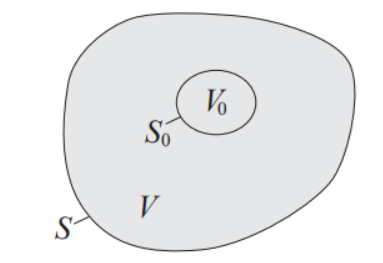
\includegraphics [height=2 in]{eigstress1}
   \caption{Representation of matrix and inclusion. This image is taken from \cite{stanford_notes}.}
   \label{fig:eigstress1}
\end{figure}

However, the inclusion is surrounded by a matrix; hence, it cannot achieve the eigenstrain and zero stress state. Instead, the inclusion and the matrix experience an elastic stress field and some displacement from the original position. Eshelby’s inclusion problem is to solve stress, strain, and displacement fields in the inclusion and the matrix. Eshelby also showed that the problem could be elegantly solved by the superposition principle of linear elasticity and Green’s function \cite{stanford_notes}.

\section{Solution to Eshelby's Inclusion Problem}
\paragraph{}
Eshelby solved the inclusion problem through a virtual experiment. The steps of the experiment are as follows:
\begin{enumerate}

    \item Remove the inclusion from the matrix and apply no force to the inclusion and the matrix. Let the inclusion relax to attain the eigenstrain under zero stress.
        \begin{figure}[H]
            \centering
            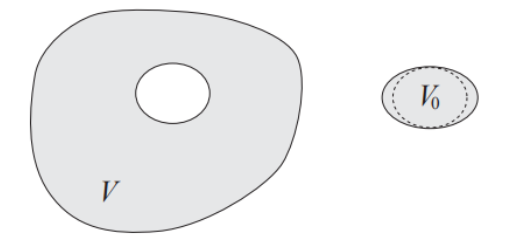
\includegraphics [height=2 in]{eigstress2}
            \caption{Representation of matrix and inclusion after step 1. This image is taken from \cite{stanford_notes}.}
            \label{fig:eigstress2}
        \end{figure}
        \begin{table}[H]
            \centering
            \begin{tabular}{|c|c|}
                \hline
                \textbf{Matrix} & \textbf{Inclusion} \\
                \hline
                $e_{ij} = 0$ & $e_{ij} = e^{*}_{ij}$ \\
                $\sigma_{ij} = 0$ & $\sigma_{ij} = 0$ \\
                $u_{i} = 0$ & $u_{i} = e^{*}_{ij}x_{j}$ \\
                \hline
            \end{tabular}
            \caption{Strain, stress, and displacement fields in matrix and inclusion after step 1. This table is taken from \cite{stanford_notes}.}
            \label{tab:step1}
        \end{table}

    \item Apply surface tension $T$ to the inclusion so that it returns to its original shape. The elastic strain due to the surface traction should exactly cancel the eigenstrain.
        \begin{figure}[H]
            \centering
            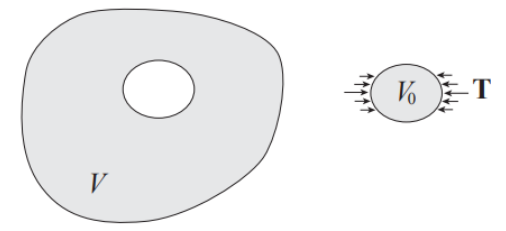
\includegraphics [height=2 in]{eigstress3}
            \caption{Representation of matrix and inclusion after step 2. This image is taken from \cite{stanford_notes}.}
            \label{fig:eigstress3}
        \end{figure}
        \begin{table}[H]
            \centering
            \begin{tabular}{|c|c|}
                \hline
                \textbf{Matrix} & \textbf{Inclusion} \\
                \hline
                $e_{ij} = 0$ & $e_{ij} = e^{el}_{ij} + e^{*}_{ij} = 0$ \\
                $\sigma_{ij} = 0$ & $\sigma_{ij} = C_{ijkl}e^{el}_{ij} = -C_{ijkl}e^{*}_{ij} = -\sigma^{*}_{ij}$ \\
                $u_{i} = 0$ & $u_{i} = 0$ \\
                \hline
            \end{tabular}
            \caption{Strain, stress, and displacement fields in matrix and inclusion after step 2. This table is taken from \cite{stanford_notes}.}
            \label{tab:step2}
        \end{table}

    \item Put the inclusion back in the matrix, but keep the surface traction forces. Since the force is not removed, there is no change in stress, strain and displacement fields.
        \begin{figure}[H]
            \centering
            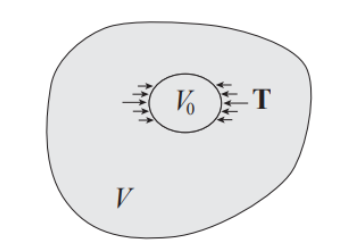
\includegraphics [height=2 in]{eigstress4}
            \caption{Representation of matrix and inclusion after step 3. This image is taken from \cite{stanford_notes}.}
            \label{fig:eigstress4}
        \end{figure}

    \item Now remove the force $T$ from the inclusion surface. This leads us to the initial problem configuration. The inclusion applies a force $F$ equal in magnitude to $T$ but opposite in direction.
        \begin{figure}[H]
            \centering
            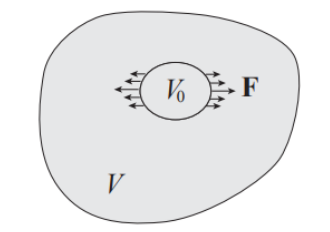
\includegraphics [height=2 in]{eigstress5}
            \caption{Representation of matrix and inclusion after step 4. This image is taken from \cite{stanford_notes}.}
            \label{fig:eigstress5}
        \end{figure}

        Let $u^{c}_{i}(x)$ be the displacement field in response to the force $F$. $u^{c}_{i}(x)$ is called the constrained displacement field. The displacement, strain, and stress fields are expressed in terms of Greens' function as follows:

        \begin{equation}
            u^{c}_{i}(x) = \int_{S_{0}} \sigma_{lk}^{*} n_{k}(x^{'}) G_{il,j}(x,x^{'})dS(x^{'})
        \end{equation}
        \begin{equation}
            e^{c}_{ij}(x) = \frac{1}{2} (u^{c}_{i,j} + u^{c}_{j,i}) = \int_{S_{0}} \sigma_{lk}^{*} n_{k}(x^{'}) [G_{il,j}(x,x^{'}) + G_{jl,i}(x,x^{'})]dS(x^{'})
        \end{equation}
        \begin{equation}
            \sigma^{c}_{ij}(x) = C_{ijkl}e^{c}_{ij}(x)
        \end{equation}

        \begin{table}[H]
            \centering
            \begin{tabular}{|c|c|}
                \hline
                \textbf{Matrix} & \textbf{Inclusion} \\
                \hline
                $e_{ij} = e^{c}_{ij}$ & $e_{ij} = e^{c}_{ij}$ \\
                $\sigma_{ij} = \sigma^{c}_{ij}$ & $\sigma_{ij} = \sigma^{c}_{ij} - \sigma^{*}_{ij} = C_{ijkl}(e^{c}_{ij} - e^{*}_{ij}) $ \\
                $u_{i} = u_{i}^{c}$ & $u_{i} = u_{i}^{c}$ \\
                \hline
            \end{tabular}
            \caption{Strain, stress, and displacement fields in matrix and inclusion after step 4. This image is taken from \cite{stanford_notes}.}
            \label{tab:step4}
        \end{table}

        The constrained field needs to be determined everywhere in the matrix and inclusion to obtain explicit expressions for stress and strain fields. A fourth order tensor, known as Eshelby's tensor $S_{ijkl}$ is defined, relating constrained strain to eigenstrain.

        \begin{equation}
            e^{c}_{ij} = S_{ijkl}e^{*}_{ij}
        \end{equation}

        Eshelby's tensor is a function of space; however, for an ellipsoidal inclusion in a homogeneous infinite matrix, the tensor is a constant, making the stress and strain fields uniform inside the inclusion \cite{stanford_notes}.
\end{enumerate}

\chapter{Literature Review}
\paragraph{}
A literature review was done to study the approaches to solving Eshelby’s inclusion problem. It turns out that there are multiple methods/approaches to solving Eshelby’s inclusion problem; prominent amongst them are the analytical solution, FFT-based solutions, and finite difference method (FDM) solution. The software implementations of these three solutions to Eshelby’s inclusion problem are studied. The software implementations are
\begin{enumerate}
    \item Analytical Solution
    \begin{enumerate}
        \item 2D Case (Work of M. P. Gururajan, based on work of M. A. Jaswon and R. D. Bhargava) \cite{jaswon_bhargava_1961}
        \item 3D Homogeneous Case (Based on the book by T. Mura, Micromechanics of Defects in Solids) \cite{mura1987micromechanics}
        \item 3D In-homogeneous Case (Based on the book by T. Mura, Micromechanics of Defects in Solids) \cite{mura1987micromechanics}
    \end{enumerate}
    \item Fast Fourier Transform Solution (Ph.D. thesis of M. P. Gururajan) \cite{Guru_thesis}
    \item Alamo Solution (Open-source framework based on AMReX) \cite{Runnels_2021}
\end{enumerate}

\section{Analytical Solution}
\subsection{2D Case}
\paragraph{}
M.A. Jaswon and R.D. Bhargava obtained an analytical solution to the Eshelby inclusion problem through the force point method and complex variable formalism \cite{jaswon_bhargava_1961}. The program is written in C language. The inputs provided to the program are the Poisson ratio, major and minor axes of the elliptical inclusion, elasticity moduli of the matrix, and the inclusion and the components of strain. Eigenstrains are calculated in the first part of the program. Stress fields are calculated in the second part of the program and stored in a file. A Python file reads the data file, and the stress field data is plotted.

For deriving the equations for stress fields, the coordinate axes are rotated counter-clockwise through an angle $\theta$ such that the axes are now oriented in principal directions \cite{jaswon_bhargava_1961}. The change in stress notations and co-relation between stresses of different notations is given as follows:

\begin{equation}
    p_{\xi\xi} + p_{\eta\eta} = p_{11} + p_{22}
\end{equation}
\begin{equation}
    p_{\xi\xi} - p_{\eta\eta} + 2ip_{\xi\eta} = (p_{22} - p_{11} + 2ip_{12})e^{2i\theta}
\end{equation}
\begin{equation}
    u_{\xi} + iu_{\eta} = (u_{1} + iu_{2})e^{-i\theta}
\end{equation}
Here $p_{\xi\xi}$ and $p_{\eta\eta}$ represent stress in X and Y directions, respectively. $p_{11}$ and $ p_{22}$ represent stresses in principal directions, respectively.
The equations for stress inside the inclusion are given as follows:
\begin{equation}
    p_{11} = \frac{-4\mu a}{(1+\kappa)(a+b)} \left( \frac{(2a+b)E^{0}_{11} + bE^0_{22}}{a+b} \right)
\end{equation}
\begin{equation}
    p_{22} = \frac{-4\mu b}{(1+\kappa)(a+b)} \left(\frac{aE^{0}_{11} + (a+2b)E^0_{22}}{a+b}\right)
\end{equation}
\begin{equation}
    p_{12} = \frac{-8\mu abE^0_{12}}{(1+\kappa)(a+b)^2}
\end{equation}
The equations for principal stress outside the inclusion are given as follows:
\begin{equation}
    p_{\xi\xi} + p_{\eta\eta} = \frac{8\mu}{\kappa + 1} \frac{ab}{c^2} \left(1 - \frac{sinh (2\xi)}{cosh (2\xi) - cos (2\eta)}\right) (E^0_{11} - E^0_{22})
\end{equation}
\begin{equation}
    p_{\xi\xi} - p_{\eta\eta} + 2ip_{\xi\eta} = \frac{8\mu}{\kappa + 1} \frac{ab}{c^2} \left(\frac{AE^0_{11} + BE^0_{22}}{cosh (2\xi) - cos (2\eta)}\right)
\end{equation}
\begin{equation}
    A = \left( cosh(2\xi) - \frac{a^2 + b^2}{c^2} \right) coth(\xi + i\eta) - sinh(2\xi) + \frac{2a^2}{c^2}[1-e^{-2(\xi + i\eta)}]
\end{equation}
\begin{equation}
    B = -\left( cosh(2\xi) - \frac{a^2 + b^2}{c^2} \right) coth(\xi + i\eta) + sinh(2\xi) - \frac{2b^2}{c^2}[1-e^{-2(\xi + i\eta)}]
\end{equation}

The equations for shear stress outside the inclusion are given as follows:
\begin{equation}
    p_{\xi\xi} + p_{\eta\eta} = -\frac{8\mu E^0_{12}}{\kappa + 1} \frac{2ab}{c^2} \frac{sin (2\eta)}{cosh (2\xi) - cos (2\eta)}
\end{equation}
\begin{equation}
    p_{\xi\xi} - p_{\eta\eta} + 2ip_{\xi\eta} = i\frac{8\mu E^0_{12}}{\kappa + 1} \frac{2ab}{c^2} \frac{A + iB}{cosh (2\xi) - cos (2\eta)}
\end{equation}
\begin{equation}
    A + iB = \left(cosh(2\xi) - \frac{a^2 + b^2}{c^2}\right)coth(\xi + i\eta)   - sinh(2\xi) + \frac{a^2 + b^2}{c^2} [1-e^{-2(\xi + i\eta)}]
\end{equation}
The principal and shear stresses are added together to get the final stresses.

\subsection{3D Homogeneous Case}
\paragraph{}
An ellipsoidal inclusion $\Omega$ is considered in an isotropic infinite body. Eigenstrains given are assumed to be uniform (constant). For general eigenstrains, the solution was arrived upon by Eshelby in his papers in 1957,1959, and 1961 \cite{mura1987micromechanics}. Expressions for solutions are different for points inside the inclusion and points outside the inclusion. The solution to both can be found explicitly for the isotropic case. Eshelby's most valuable result is that the strain and stress fields become uniform for the interior points.

\subsubsection{Interior Points}
\paragraph{}
To find the solution to define and evaluate two integrals, which are given by
\begin{equation}
    I_{1} = \frac{4\pi a_1 a_2 a_3}{(a_{1}^{2} - a_{2}^{2})(a_{1}^{2} - a_{3}^{2})^{\frac{1}{2}}} \left(F(\theta, k) - E(\theta,k)\right)
\end{equation}
\begin{equation}
    I_{3} = \frac{4\pi a_1 a_2 a_3}{(a_{2}^{2} - a_{3}^{2})(a_{1}^{2} - a_{3}^{2})^{\frac{1}{2}}} \left(\frac{a_2 (a_{1}^{2} - a_{3}^{2})^{\frac{1}{2}}}{a_1 a_3} - E(\theta,k)\right)
\end{equation}
where
\begin{equation}
    F(\theta, k) = \int_{0}^{\theta} \frac{d\omega}{(1 - k^2 sin^2 \omega)^{1/2}}
    \label{Felliptic}
\end{equation}
\begin{equation}
    E(\theta, k) = \int_{0}^{\theta} (1 - k^2 sin^2 \omega)^{1/2} d\omega
    \label{Eelliptic}
\end{equation}

\begin{equation}
    \theta = sin^{-1}( 1 - a_{3}^{2}/a_{1}^{2})^{1/2} ,\hspace{5mm}  k = \left(\frac{a_{1}^{2} - a_{2}^{2}}{a_{1}^{2} - a_{3}^{2}}\right) ^{1/2}
\end{equation}
$a_1$, $a_2$, and $a_3$ are radii of the ellipsoidal inclusion, with an assumption that $a_1 > a_2 > a_3$. Here the integral $F$ is also known as First Order Elliptic Integral and $E$ is known as second order elliptic integral.\\

After evaluating $I_1$ and $I_3$, $I_2$ can be evaluated by using the equation
\begin{equation}
    I_1 + I_2 + I_3 = 4\pi
\end{equation}
After evaluating $I_2$, the integral $I_{12}$ can be evaluated by using the equation
\begin{equation}
    I_{12} = (I_2 - I_1)/(a_{1}^{2} - a_{2}^{2})
\end{equation}
After evaluating the integral $I_{12}$, the integrals $I_{11}$ and $I_{13}$ can be evaluated by solving simultaneous equations
\begin{equation}
    3I_{11} + I_{12} + I_{13} = 4\pi /a_{1}^{2}
\end{equation}
\begin{equation}
    3a_{1}^{2}I_{11} + a_{2}^{2}i_{12} + a_{3}^{2}I_{13} = 3I_1
\end{equation}

After evaluating all the integrals, the equations for stress are given as follows
\begin{align}
    %\sigma_{11}/2\mu =  &\left[\frac{a_{1}^{2}}{8\pi (1-\nu)} \left(\frac{1 - \nu}{1 - 2\nu}3I_{11} + \frac{\nu}{1-2\nu}(I_{21} + I_{31})\right) \nonumber \\
    %&+ \frac{1-2\nu}{8\pi (1-\nu)} \left( \frac{1-\nu}{1-2\nu}I_1 - \frac{\nu}{1-2\nu}(I_2 + I_3)\right) - \frac{1-\nu}{1-2\nu} \right] \epsilon_{11}^{*}
    \frac{\sigma_{11}}{2\mu} &= \left[\frac{a_{1}^{2}}{8\pi (1-\nu)} \left(\frac{1 - \nu}{1 - 2\nu}3I_{11} + \frac{\nu}{1-2\nu}(I_{21} + I_{31})\right) \right. \nonumber \\
    &+  \left. \frac{1-2\nu}{8\pi (1-\nu)} \left( \frac{1-\nu}{1-2\nu}I_1 - \frac{\nu}{1-2\nu}(I_2 + I_3)\right)  -\frac{1-\nu}{1-2\nu} \right] \epsilon_{11}^{*} \nonumber \\
    &+ \left[\frac{a_{2}^{2}}{8\pi (1-\nu)} \left(\frac{1 - \nu}{1 - 2\nu}I_{12} + \frac{\nu}{1-2\nu}(3I_{22} + I_{32})\right) \right. \nonumber \\
    &-  \left. \frac{1-2\nu}{8\pi (1-\nu)} \left( \frac{1-\nu}{1-2\nu}I_1 - \frac{\nu}{1-2\nu}(I_2 - I_3)\right)  -\frac{\nu}{1-2\nu} \right] \epsilon_{22}^{*} \nonumber \\
    &+ \left[\frac{a_{3}^{2}}{8\pi (1-\nu)} \left(\frac{1 - \nu}{1 - 2\nu}I_{13} + \frac{\nu}{1-2\nu}(3I_{33} + I_{23})\right) \right. \nonumber \\
    &-  \left. \frac{1-2\nu}{8\pi (1-\nu)} \left( \frac{1-\nu}{1-2\nu}I_1 - \frac{\nu}{1-2\nu}(I_3 - I_2)\right)  -\frac{\nu}{1-2\nu} \right] \epsilon_{11}^{*}
\end{align}
\begin{equation}
    \sigma_{12}/2\mu = \left( \frac{a_{1}^{2} + a_{2}^{2}}{8\pi (1-\nu)}I_{12} + \frac{1-2\nu}{8\pi (1-\nu)}(I_1 + I_2) -1 \right) \epsilon_{12}^{*}
\end{equation}

Other components of stress are obtained by the cyclic permutation of (1,2,3).

\subsubsection{Exterior Points}
\paragraph{}
Unlike interior points, the stress and strain fields in the exterior of the inclusion are not constant; hence, they need to be computed individually at every point of interest. Computation of stress at an exterior point involves computation of the lambda parameter, the elliptic integrals, derivatives of the lambda parameter and the elliptic integrals, the $S_{ijkl}$ tensor, the $D_{ijkl}$ tensor, the strain fields and then ultimately stress field. \\

The elliptic integrals are given by 
\begin{equation}
    I(\lambda) = 2\pi a_1 a_2 a_3 \int_{\lambda}^{\infty} \frac{ds}{\Delta (s)}
\end{equation}
\begin{equation}
    I_{i}(\lambda) = 2\pi a_1 a_2 a_3 \int_{\lambda}^{\infty} \frac{ds}{(a_{i}^{2} + s) \Delta (s)}
\end{equation}
\begin{equation}
    I_{ij}(\lambda) = 2\pi a_1 a_2 a_3 \int_{\lambda}^{\infty} \frac{ds}{(a_{i}^{2} + s)(a_{j}^{2} + s) \Delta (s)}
\end{equation}
where $\Delta(s) = ((a_{1}^{2} + s)(a_{2}^{2} + s)(a_{3}^{2} + s))^{1/2}$, and $\lambda$ is the largest positive root of the equation
\begin{equation}
    \frac{x_{1}^{2}}{(a_{1}^{2} + \lambda)} + \frac{x_{2}^{2}}{(a_{2}^{2} + \lambda)} + \frac{x_{3}^{2}}{(a_{3}^{2} + \lambda)} = 1
    \label{eq:lambda_eq}
\end{equation}
for an exterior point $x$. For interior points, $\lambda = 0$.

Since $\lambda$ is a root of the equation \ref{eq:lambda_eq}, differentiating the equation w.r.t. $x_{l}$ would give us derivative of $\lambda$ which is $\lambda_{,l}$.

\begin{equation}
    \lambda_{,l} = \frac{2x_{l}}{a_{L}^{2} + \lambda} / \frac{x_i x_i}{(a_{I}^{2} + \lambda)^2}
    \label{lambda_der}
\end{equation}

Note that repeated lower case indices are summed up from 1 to 3, but the upper case indices take on the same number as the corresponding lower case index but are not summed up. For example, in equation \ref{lambda_der},
\begin{equation}
    \frac{x_i x_i}{(a_{I}^{2} + \lambda)^2} = \frac{x_{1}^{2}}{(a_{1}^{2} + \lambda)^2} + \frac{x_{2}^{2}}{(a_{2}^{2} + \lambda)^2} + \frac{x_{3}^{2}}{(a_{3}^{2} + \lambda)^2}
\end{equation}

Similarly, the double derivative of lambda can be calculated by differentiating the equation \ref{lambda_der}. The double derivatives are required to compute $D_{ijkl}$ tensor.
\begin{equation}
    \lambda_{,ij} = \left({\frac{2 x_r x_r}{(a_{R}^{2} + \lambda)^2} \lambda_{,i} \lambda_{,j} - \frac{2x_i}{(a_{i}^{2} + \lambda)^2} \lambda_{,j} - \frac{2x_j}{(a_{j}^{2} + \lambda)^2} \lambda_{,i}}\right) / \frac{x_s x_s}{(a_{S}^{2} + \lambda)^2}
\end{equation}

These above-mentioned derivatives of $\lambda$ parameter are then used in calculations of derivatives of elliptic integrals. The elliptic integrals are independent of $x$ with only the lower bound $\lambda$, dependent on $x$. Hence, the derivatives of elliptic integrals can be reduced to derivatives of $\lambda$ as follows:

\begin{equation}
    I_{i,j}(\lambda) = \frac{-2\pi a_1 a_2 a_3}{(a_{i}^{2} + \lambda) \Delta (\lambda)} \cdot \lambda_{,j}
\end{equation}
\begin{equation}
    I_{ij,k}(\lambda) = \frac{-2\pi a_1 a_2 a_3}{(a_{i}^{2} + \lambda)(a_{j}^{2} + \lambda) \Delta (\lambda)} \cdot \lambda_{,k}
\end{equation}
where 
\begin{equation}
    \Delta (\lambda) = \left((a_{1}^{2} + \lambda)(a_{2}^{2} + \lambda)(a_{3}^{2} + \lambda)\right)^{1/2}
\end{equation}

Double derivatives of elliptic integrals are given as follows:
\begin{equation}
    I_{i,jk}(\lambda) = \frac{-2\pi a_1 a_2 a_3}{(a_{i}^{2} + \lambda) \Delta (\lambda)} \left[\lambda_{,jk} - \lambda_{,j}\lambda_{,k}\left(\frac{1}{(a_{j}^{2} + \lambda)} + \frac{T_r}{2} \right)  \right]
\end{equation}
\begin{equation}
    I_{ij,kl}(\lambda) = \frac{-2\pi a_1 a_2 a_3}{(a_{i}^{2} + \lambda)(a_{j}^{2} + \lambda) \Delta (\lambda)} \left[\lambda_{,kl} - \lambda_{,k}\lambda_{,l}\left(\frac{1}{(a_{i}^{2} + \lambda)} + \frac{1}{(a_{j}^{2} + \lambda)} + \frac{T_r}{2} \right)  \right]
\end{equation}
where
\begin{equation}
    T_r = \frac{1}{a_{1}^{2} + \lambda} + \frac{1}{a_{2}^{2} + \lambda} + \frac{1}{a_{3}^{2} + \lambda}
\end{equation}

After computing all the elliptic integrals and their derivatives, $S_{ijkl}$ tensor is computed using the following equation:
\begin{align}
    8\pi &(1-\nu)S_{ijkl}(\lambda) = \delta_{ij}\delta_{kl}\left[2\nu I_{I}(\lambda) - I_{K}(\lambda) + a_{I}^{2} I_{KI}(\lambda) \right] \nonumber \\
    &+ (\delta_{ik}\delta_{jl} + \delta_{jk}\delta_{il})\left(a_{I}^2 I_{IJ}(\lambda) - I_{J}(\lambda) + (1-v)\left[I_{K}(\lambda) + I_{L}(\lambda)  \right]\right)
\end{align}

After computing $S_{ijkl}$ tensor, $D_{ijkl}$ tensor is computed using the following equation.
\begin{align}
    8\pi&(1-\nu)D_{ijkl}(x) = 8\pi(1-\nu)S_{ijkl}(\lambda) + 2\nu\delta_{kl}x_{i}I_{I,j}(\lambda) \nonumber \\
    &+(1-\nu)\left[\delta_{il}x_{k}I_{K,j}(\lambda) + \delta_{jl}x_{k}I_{K,i}(\lambda) + \delta_{ik}x_{l}I_{L,j}(\lambda) + \delta_{jk}x_{l}I_{L,i}(\lambda)\right] \nonumber \\
    &-\delta_{ij}x_{k}\left[I_{K}(\lambda) -a_{I}^{2}I_{KI}(\lambda)\right]_{,l} - \left(\delta_{ik}x_{j} + \delta_{jk}x_{i}\right)\left[I_{J}(\lambda) - a_{I}^{2}I_{IJ}(\lambda)\right]_{,l} \nonumber \\
    &-\left(\delta_{il}x_{j} + \delta_{jl}x_{i}\right)\left[I_{J}(\lambda) - a_{I}^{2}I_{IJ}(\lambda) \right]_(,k) - x_{i}x_{j}\left[I_{J}(\lambda) - a_{I}^{2}I_{IJ}(\lambda)\right]_{,lk}
\end{align}

The above equations for $S_{ijkl}$ and $D_{ijkl}$ hold true for both interior and exterior. In the interior of inclusion, $\lambda = 0$, and all the gradients of $\lambda$, $I_i$ and $I_{ij}$ vanish. Then $D_{ijkl}$ becomes $S_{ijkl}(0)$ \\

The induced strain field outside can be found using the following equation
\begin{equation}
    \epsilon_{ij}(x) = D_{ijkl}\epsilon_{kl}^{*}
    \label{eq:epsilon}
\end{equation}
where $\epsilon_{kl}^{*}$ is eigenstrain. \\

For finding the stress field, we now use Hooke's Law
\begin{equation}
    \sigma_{ij} = \frac{E\nu}{(1+\nu)(1-2\nu)}\delta_{ij}\epsilon_{kk} + \frac{E}{1+\nu}\epsilon_{ij}
    \label{eq:stress}
\end{equation}

We can use equation \ref{eq:stress} to find stress inside the inclusion by defining strain inside as
\begin{equation}
    \epsilon_{ij}(x) = D_{ijkl}\epsilon_{kl}^{*} - \epsilon_{ij}^{*}
\end{equation}

\subsection{3D In-homogeneous Case}
\paragraph{}
The elastic moduli for the inclusion and matrix are the same in a homogeneous case. In an in-homogeneous case, the elastic moduli are different. In such in-homogeneous cases, the results obtained from the homogeneous case can be used by using the \textbf{Equivalent Inclusion Method}.\\

The Equivalent Inclusion Method simulates the stress disturbance by using the eigenstrain resulting from the in-homogeneous inclusion. A strain $\epsilon_{ij}^{*}$ is introduced arbitrarily to simulate the in-homogeneity. \\

Consider an inclusion with elasticity $C_{ijkl}^{*}$ inside a matrix with elasticity $C_{ijkl}$. Therefore the necessary and sufficient condition for the equivalency of the stresses and strains in the in-homogeneous inclusion is 
\begin{equation}
    C_{ijkl}^{*}(\epsilon_{kl}^{0} + \epsilon_{kl}) = C_{ijkl}(\epsilon_{kl}^{0} + \epsilon_{kl} - \epsilon^{*}_{kl})
    \label{equi1}
\end{equation}
However, it is known that $\epsilon_{kl}$ in the above equation can be obtained as a function of $\epsilon^{*}_{kl}$.
\begin{equation}
    \epsilon_{kl} = S_{klmn}\epsilon_{mn}^{*}
    \label{equi2}
\end{equation}
Substituting equation \ref{equi2} in \ref{equi1} leads to,
\begin{equation}
    C_{ijkl}^{*}(\epsilon_{kl}^{0} + S_{klmn}\epsilon_{mn}^{*}) = C_{ijkl}(\epsilon_{kl}^{0} + S_{klmn}\epsilon_{mn}^{*} - \epsilon^{*}_{kl})
\end{equation}
from which the six unknowns, $\epsilon_{ij}^{*}$, can be determined. \\

Sometimes the inhomogeneity may involve its own eigenstrain, $\epsilon_{ij}^{p}$. In such case, the equation \ref{equi1} transforms as,
\begin{equation}
    C_{ijkl}^{*}(\epsilon_{kl}^{0} + \epsilon_{kl} - \epsilon_{kl}^{p}) = C_{ijkl}(\epsilon_{kl}^{0} + \epsilon_{kl} - \epsilon^{*}_{kl} - \epsilon_{kl}^{p})
    \label{equi3}
\end{equation}
Equation \ref{equi2} transforms as
\begin{equation}
    \epsilon_{kl} = S_{klmn}(\epsilon_{mn}^{p} + \epsilon_{mn}^{*}) = S_{klmn}\epsilon_{mn}^{**}
    \label{equi4}
\end{equation}
where,
\begin{equation}
    \epsilon_{mn}^{**} = \epsilon_{mn}^{p} + \epsilon_{mn}^{*}
\end{equation}
Substituting equation \ref{equi4} in \ref{equi3} yields,
\begin{equation}
    C_{ijkl}^{*}(\epsilon_{kl}^{0} + S_{klmn}\epsilon_{mn}^{**} - \epsilon_{kl}^{p}) = C_{ijkl}(\epsilon_{kl}^{0} + S_{klmn}\epsilon_{mn}^{**} - \epsilon^{**}_{kl})
\end{equation}

In case of isotropic materials, equation \ref{equi3} can be written as,
\begin{equation}
   2\mu^{*}(\epsilon_{ij}^{0} + \epsilon_{ij} - \epsilon_{ij}^{p}) +\lambda^{*}\delta_{ij}(\epsilon_{kk}^{0} + \epsilon_{kk} - \epsilon_{kk}^{p}) = 2\mu(\epsilon_{ij}^{0} + \epsilon_{ij} - \epsilon_{ij}^{**}) +\lambda^{*}\delta_{ij}(\epsilon_{kk}^{0} + \epsilon_{kk} - \epsilon_{kk}^{**})
   \label{equi5}
\end{equation}
where $\lambda^*$, $\mu^*$ and $\lambda$, $\mu$ are the Lamé constants in the inhomogeneity and the matrix.

The equation \ref{equi5} can be equivalently written by using deviatoric strains. The deviatoric strains are,
\begin{align}
    '\epsilon_{ij}^{0} &= \epsilon_{ij}^{0} - \delta_{ij}\epsilon_{kk}^{0}/3 \nonumber \\
    '\epsilon_{ij}^{p} &= \epsilon_{ij}^{p} - \delta_{ij}\epsilon_{kk}^{p}/3 \nonumber \\
    '\epsilon_{ij}^{**} &= \epsilon_{ij}^{**} - \delta_{ij}\epsilon_{kk}^{**}/3 \nonumber \\
    '\epsilon_{ij} &= \epsilon_{ij} - \delta_{ij}\epsilon_{kk}/3
\end{align}
The equation \ref{equi5} can be written using deviatoric strains as
\begin{align}
    2\mu^{*}('\epsilon_{ij}^{0} + '\epsilon_{ij} - '\epsilon_{ij}^{p}) &= 2\mu('\epsilon_{ij}^{0} + '\epsilon_{ij} - '\epsilon_{ij}^{**}) \nonumber \\
    K^{*}(\epsilon_{kk}^{0} + \epsilon_{kk} - \epsilon_{kk}^{p}) &= K(\epsilon_{kk}^{0} + \epsilon_{kk} - \epsilon_{kk}^{**})
    \label{equi6}
\end{align}
where
\begin{align}
    K &= \lambda + \frac{2\mu}{3} = \frac{E}{3(1 - 2\nu)} \nonumber \\
    E &= 2(1+\nu)\mu \nonumber \\
    \lambda &= \frac{2\mu\nu}{1-2\nu}
\end{align}

The shear components of $\epsilon^{**}_{ij}$ can be obtained from the first equation of \ref{equi6}.
\begin{align}
    \epsilon_{12}^{**} = \frac{2(\mu - \mu^{*})\epsilon_{12}^{0} + 2\mu^{*}\epsilon_{12}^{p}}{4(\mu^{*} - \mu)S_{1212} + 2\mu} \nonumber \\
    \epsilon_{23}^{**} = \frac{2(\mu - \mu^{*})\epsilon_{23}^{0} + 2\mu^{*}\epsilon_{23}^{p}}{4(\mu^{*} - \mu)S_{2323} + 2\mu} \nonumber \\
    \epsilon_{31}^{**} = \frac{2(\mu - \mu^{*})\epsilon_{31}^{0} + 2\mu^{*}\epsilon_{31}^{p}}{4(\mu^{*} - \mu)S_{3131} + 2\mu}
\end{align}

To obtain the normal components of strain, the second equation of \ref{equi6} can be rearranged, and a system of linear equations consisting of three equations and three variables can be set up.
\begin{equation}
\small
\begin{bmatrix}
(1-t)S_{1111} - 1 & (1-t)S_{1122} & (1-t)S_{1133} \\
(1-t)S_{2211} & (1-t)S_{2222} - 1 & (1-t)S_{2233} \\
(1-t)S_{3311} & (1-t)S_{3322} & (1-t)S_{3333} \\
\end{bmatrix}
\begin{bmatrix}
    \epsilon_{11}^{*} \\
    \epsilon_{22}^{*} \\
    \epsilon_{33}^{*} \\
\end{bmatrix} = 
\begin{bmatrix}
    (t-1)\epsilon_{11}^{0} - t\epsilon_{11}^{p} - (1-t)S_{11mn}\epsilon_{mn}^{**} \\
    (t-1)\epsilon_{22}^{0} - t\epsilon_{22}^{p} - (1-t)S_{22mn}\epsilon_{mn}^{**} \\
    (t-1)\epsilon_{33}^{0} - t\epsilon_{33}^{p} - (1-t)S_{33mn}\epsilon_{mn}^{**} \\
\end{bmatrix}
\end{equation}
where, $t = \frac{K^*}{K}$ \\


\textbf{NOTE: IN RHS OF ABOVE EQUATION, THE SUMMATION $S_{11mn}\epsilon_{mn}^{**}$ AND OTHERS NEED TO BE DONE ON CONDITION $m \neq n$} \\

After evaluating all the strain components, equation \ref{eq:stress} can be used to find the stress fields inside and outside the inclusion.

\section{Fast Fourier Transform (FFT) Solution}
\paragraph{}
Fast Fourier Transform (FFT) based iterative method is used to solve mechanical equilibrium equations under predefined traction conditions, as discussed in the Ph.D. thesis of M.P. Gururajan \cite{Guru_thesis}. This implementation is validated against an analytical solution and is found to be coherent. The program is written in C language. The inputs provided are the Poisson ratio, major and minor axes of the elliptical inclusion, elasticity constants ($C_{11}$, $C_{12}$, $C_{44}$) of the matrix, and the inclusion, the components of strain, system simulation size, grid cell size and time information for which the simulation is to be run.

\section{Alamo Solution}
\paragraph{}
Traditionally, Finite Element Methods (FEM) were used for elasticity calculations. FEM is renowned for its ability to handle meshes of complex geometry using iso-parametric elements and weak formulation, which avoids the computation of second derivatives. However, for elasticity, problems where the topology varies by space and time (e.g., Microstructure Evolution), either Adaptive Mesh Refinements (AMR) or complete re-meshing is required. Block Structured AMR (BSAMR) can be useful in such cases where topology varies because of its scaling properties. Alamo is an implementation of such a BSAMR called AMReX and the multigrid-solver. It is shown by Runnels B. et al. that equation of BSAMR can be solved efficiently by the finite difference method (FDM) \cite{Runnels_2021}. \\


BSAMR generated finer meshes where the properties’ changes are more significant than their surroundings. A diffuse indicator function is defined to quantify these, and a criterion is set based on the difference in the diffuse indicator function and the spatial distance. Where the criterion is met, blocks are refined further by BSAMR \cite{Runnels_2021}. The diffuse indicator is given by :
\begin{equation}
    \eta_{\epsilon}(x) = \frac{1}{2} \left(1 - erf\left(\frac{x^TAx}{2\epsilon \left|Ax\right|}\right)\right)
\end{equation}
The criterion for refining of blocks by BSAMR is given by:
\begin{equation}
    \left|\nabla \eta (x) \right|\left|\Delta x\right| > 0.01
\end{equation}

\begin{figure}[H]
    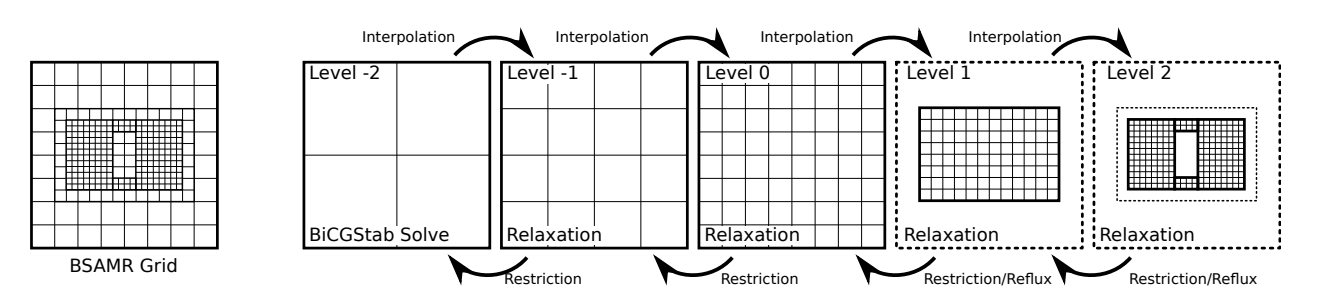
\includegraphics[width=\textwidth]{images/BSAMR Grid.png}
    \caption{Illustration of grid refining and coarsening by solver. This image is taken from \cite{Runnels_2021}}
    \label{fig:BSAMRGrid}
\end{figure}

\begin{figure}[H]
    \centering
    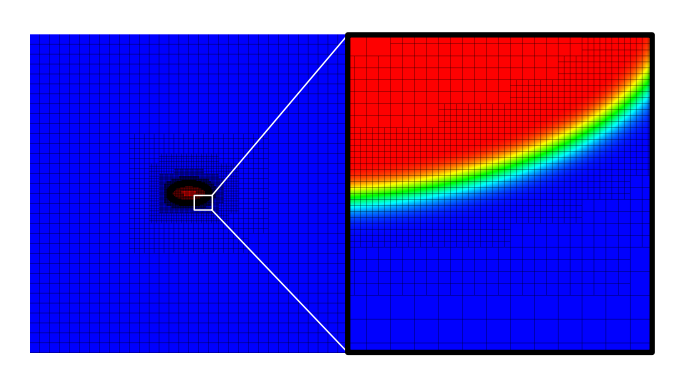
\includegraphics[height =2in]{images/Eshelbygrid.png}
    \caption{Meshing in Eshelby's inclusion problem. This image is taken from \cite{Runnels_2021}.}
    \label{fig:Eshelbygrid}
\end{figure}

The program Alamo is an open-source package developed by the Solid Mechanics Research group at the University of Colorado, Colorado Springs. The program is developed in C++ and Python Languages.\\


An implementation of the Eshelby problem is provided along with the package. The Eshelby problem is solved in the grid size of 8*8*8 units with five levels of AMR refinement. The diffuse boundary is set at 0.1 units, and the base level grid is 32*32*32. The radii of inclusion in the x, y, and z directions are 1, 0.75, and 0.5 units, respectively. The Elasticity modulus of both matrix and precipitate is 210, the Poisson ratio is 0.3, and the Eshelby strain is [0.001, 0.001, 0.001] in three principal directions. The graphical representation of the results is obtained below in Figure \ref{fig:demoplot} \cite{Runnels_2021}.

\begin{figure}[H]
    \centering
    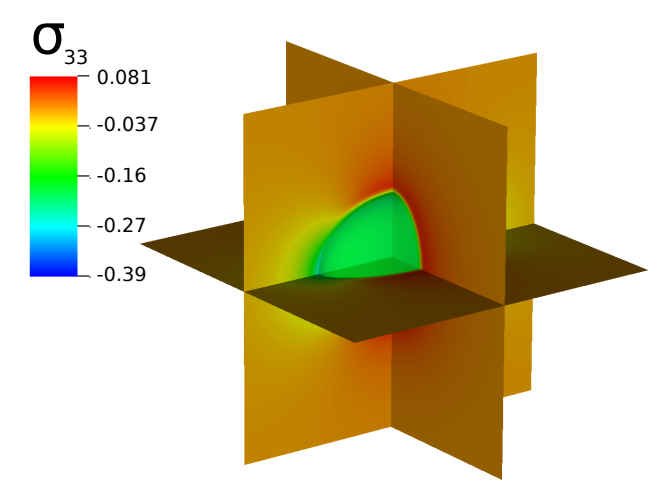
\includegraphics[height =2in]{images/demoplot.png}
    \caption{Slice plot of stress in the z direction; green ellipsoid shows the inclusion boundary.This image is taken from \cite{Runnels_2021}.}
    \label{fig:demoplot}
\end{figure}

The experiment was done in three dimensions. Alamo also supports two-dimensional simulations by suitable changes in the input file.\\


The primary reason to study the Alamo solution is to overcome a limitation of the FFT solution, wherein the FFT solution assumes a periodic boundary condition; the Alamo solution gives us the freedom to choose between a periodic or a non-periodic boundary condition.

\chapter{Implementation and Benchmarking}
\section{Operating Range of Software Implementations}
\paragraph{}
The convergence of programs and their output was observed for various combinations of elasticity modulus of inclusion and matrix. The limits to the working range were determined for all three software implementations. It was found that the Analytical solution and FFT solution worked on the entire range of ratio $[0, \infty)$ of elasticity modulus of inclusion and matrix. The ratio $\frac{E_m}{E_p}$ is 0 when $E_m$ is 0; ratio $\frac{E_m}{E_p}$ is $\infty$ when $E_p$ is 0. Some limitations were found for the Alamo solution, summarised in Tables \ref{Alamo2DValid} and \ref{Alamo3DValid}

\begin{table}[H]
    \centering
    \begin{tabular}{|c|c|c|c|c|c|}
        \hline
        & \textbf{$E_m$ = 50} &\textbf{$E_m$ = 40}&\textbf{$E_m$ = 30}&\textbf{$E_m$ = 20}&\textbf{$E_m$ = 10}\\
        \hline
        \textbf{$E_p$ = 1} & No & No & No & No & Yes\\
        \hline
        \textbf{$E_p$ = 2} & No & No & Yes & Yes & Yes\\
        \hline
        \textbf{$E_p$ = 3} & Yes & Yes & Yes & Yes & Yes\\
        \hline
        \textbf{$E_p$ = 4} & Yes & Yes & Yes & Yes & Yes\\
        \hline
        \textbf{$E_p$ = 5} & Yes & Yes & Yes & Yes & Yes\\
        \hline
        \textbf{Cutoff $E_p$} & 2.8 & 2.25 & 1.7 & 1.15 & 0.56\\
        \hline
        \textbf{$E_m$ / Cutoff $E_p$} & 17.85 & 17.77 & 17.64 & 17.39 & 17.85\\
        \hline
    \end{tabular}
    \caption{Summary of experiments done on Alamo 2D solution}
    \label{Alamo2DValid}
\end{table}

\begin{table}[H]
    \centering
    \begin{tabular}{|c|c|c|c|c|c|}
        \hline
        & \textbf{$E_m$ = 50} &\textbf{$E_m$ = 40}&\textbf{$E_m$ = 30}&\textbf{$E_m$ = 20}&\textbf{$E_m$ = 10}\\
        \hline
        \textbf{$E_p$ = 1} & No & No & No & Yes & Yes\\
        \hline
        \textbf{$E_p$ = 2} & No & Yes & Yes & Yes & Yes\\
        \hline
        \textbf{$E_p$ = 3} & Yes & Yes & Yes & Yes & Yes\\
        \hline
        \textbf{$E_p$ = 4} & Yes & Yes & Yes & Yes & Yes\\
        \hline
        \textbf{$E_p$ = 5} & Yes & Yes & Yes & Yes & Yes\\
        \hline
        \textbf{Cutoff $E_p$} & 2 & 1.6 & 1.2 & 0.8 & 0.4\\
        \hline
        \textbf{$E_m$ / Cutoff $E_p$} & 25 & 25 & 25 & 25 & 25\\
        \hline
    \end{tabular}
    \caption{Summary of experiments done on Alamo 3D solution}
    \label{Alamo3DValid}
\end{table}

The ‘Yes’ entries in Tables \ref{Alamo2DValid} and \ref{Alamo3DValid} mean that the program ran successfully. The ‘No’ entries mean the program didn’t converge or demonstrated abnormally slow convergence. The ‘Cutoff $E_p$’ term estimates the minimum value of $E_p$ for which the program converges. The ‘Cutoff $E_p$’ term is approximated to the nearest multiple of 0.05 in Table \ref{Alamo3DValid} to get accurate ‘$E_m$ / Cutoff $E_p$’ ratios. It is observed that when simulating Eshelby’s solution in 2D, the program runs successfully when the $E_m/E_p$ ratio is lesser than 17.7 (average of 5 values from table \ref{Alamo2DValid}). Similarly, when simulating in 3D, the program runs successfully when the $E_m/E_p$ ratio is lesser than 25. Poisson's ratio was kept constant at 0.3 throughout all the experiments. In this study, I have tested the convergence only. The correctness of the solution is validated in the next section.

\section{Correctness of Solutions}
\paragraph{}
FFT and Alamo software implementations are benchmarked against analytical solutions. The benchmarking is done under various cases such as
\begin{itemize}
    \item 2D vs. 3D
    \item Normal strain vs. Shear strain
    \item Homogeneous Case vs. In-homogeneous Case
    \begin{itemize}
        \item $E_m/E_p = 2$
        \item $E_m/E_p = 0.5$
    \end{itemize}
\end{itemize}
For every simulation, the following details are mentioned:
\begin{itemize}
    \item Parameters of simulation system for analytical Solution and software implementation benchmarked
    \begin{itemize}
        \item Elasticity Constants of Inclusion and Matrix
        \item Strain field
        \item System size / Grid size (if any)
        \item Any other input specified
    \end{itemize}
    \item Stress Profile Plots
    \begin{itemize}
        \item $\sigma_{xx}, \sigma_{yy}$ for 2D Normal Strain
        \item $\sigma_{xy}$ for 2D Shear Strain
        \item $\sigma_{xx}, \sigma_{yy}, \sigma_{zz}$ for 3D Normal Strain
        \item $\sigma_{xy}, \sigma_{yz}, \sigma_{zx}$ for 3D Normal Strain
    \end{itemize}
    \item Error plots in stress profiles
    \item Error parameters ($L_1$, $L_2$, $L_\infty$ errors)
    \item Other Comments (if any)
\end{itemize}

\paragraph{}
For stress and error profile plots, the x-axis is the normalized distance from the center, normalized with the ellipsoidal inclusion's semi-major axis, $a_1$. On the y-axis, stress is plotted for stress profile graphs, and absolute error in stress is plotted in error graphs. \\

Three types of error metrics are reported for every experiment. $L_1$, $L_2$ and $L_\infty$. They are given by
\begin{equation}
    e_i = \left| \sigma_{numerical} - \sigma_{analytical}\right|
\end{equation}
\begin{equation}
    L_{1}\,  error = \sum e_i
\end{equation}
\begin{equation}
    L_{2}\,  error = \sqrt{\sum e_{i}^{2}}
\end{equation}
\begin{equation}
    L_{\infty}\,  error = max(e_i)
\end{equation}

\textbf{Note on FFT Implementation}
\paragraph{}
Pure shear eigen-strains cannot be applied to FFT Solutions. As a result, benchmarking FFT solutions under pure shear conditions is impossible. This is because, FFT assumes a periodic boundary condition. Under pure shear conditions, there will be far-field residual shear stresses on the boundary of cells, and two adjacent cells cannot have the same shear force acting in the same direction on their shared boundary. \\

The inputs to the FFT implementation are elasticity constants $C_{11}, C_{12}, C_{44}$. However, I have modified the code to accept Young's modulus and Poisson's ratio as inputs. The code reads Young's modulus and Poisson's ratio, calculates $C_{11}, C_{12}$ and $C_{44}$, and then feed them to the program.
\begin{align}
    C_{11} &= \frac{E(1-\nu)}{(1+\nu)(1-2\nu)} \nonumber \\
    C_{12} &= \frac{E(\nu)}{(1+\nu)(1-2\nu)} \nonumber \\
    C_{44} &= \frac{E}{2(1+\nu)}
\end{align}

\newpage
\subsection{Benchmarking FFT Solution in 2D}

\subsubsection{Homogeneous Case - Normal Strain}
\begin{table}[H]
    \centering
    \begin{tabular}{|c|c|c|}
        \hline
        & \textbf{FFT} &\textbf{Analytical}\\
        \hline
        \textbf{$a_1$} & 50 & 50 \\
        \hline
        \textbf{$a_2$} & 25 & 25 \\
        \hline
        \textbf{$\nu$} & 0.3 & 0.3 \\
        \hline
        \textbf{$E_p$} & 210 & 210 \\
        \hline
        \textbf{$E_m$} & 210 & 210 \\
        \hline
        \textbf{$\epsilon_{11}$} & 0.001 & 0.001 \\
        \hline
        \textbf{$\epsilon_{22}$} & 0.001 & 0.001 \\
        \hline
        \textbf{$\epsilon_{12}$} & 0 & 0 \\
        \hline
        \textbf{Other} & Grid size = 1024*1024, Cell size = 1*1 &  \\
        \hline
    \end{tabular}
    \caption{Input parameters for FFT - 2D - homogeneous - normal strain}
\end{table}

\begin{figure}[htbp]
  \centering
  \subfigure[Stress plot for homogeneous - normal strain]{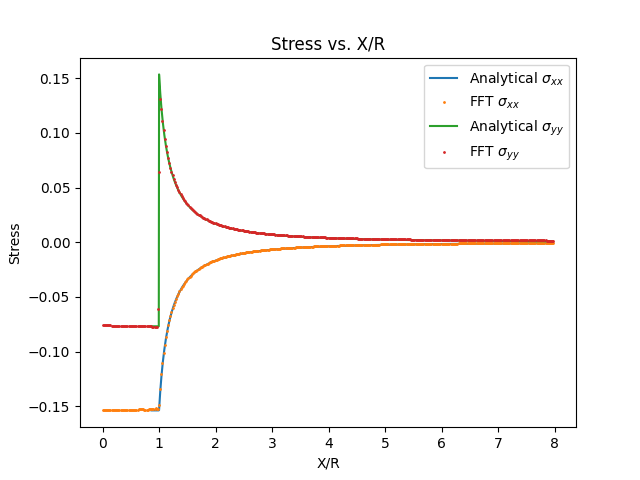
\includegraphics[width=0.45\textwidth]{images/2D_H_N_stress.png}}
  \hfill
  \subfigure[Error plot for homogeneous - normal strain]{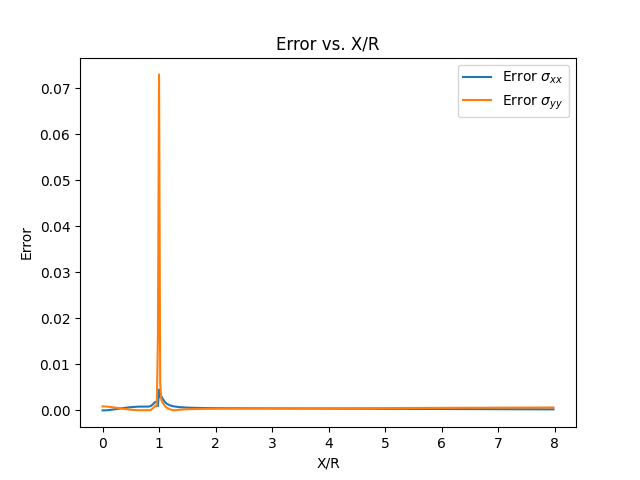
\includegraphics[width=0.45\textwidth]{images/2D_H_N_error.png}}
  \caption{Stress and error plots for FFT - 2D - homogeneous - normal strain}
\end{figure}

\begin{table}[H]
    \centering
    \begin{tabular}{|c|c|c|}
        \hline
        &\textbf{$\sigma_{11}$} &  \textbf{$\sigma_{22}$} \\
        \hline
        $L_1$ & 0.186592 & 0.283945 \\
        \hline
        $L_2$ & 0.012176 & 0.075646  \\
        \hline 
        $L_\infty$ & 0.004528 & 0.073055 \\
        \hline
    \end{tabular}
    \caption{Error in FFT - 2D - homogeneous - normal strain}
\end{table}

\paragraph{}
The input parameters, Stress profile plots, error plots, and error metrics for 2D, homogeneous case under normal strain conditions for FFT solution benchmarking are shown. Both the solutions are in good agreement. There is Low error in $\sigma_{11}$ as compared to $\sigma_{22}$, as there is a discontinuity in $\sigma_{22}$. About 25\% error in $\sigma_{22}$ concentrated near the discontinuity.


%%%%%%%%%%%%%%%%%%%%%%%%%%%%%%%%%%%%%%%%%%%%%%%%%
\newpage
\subsubsection{In-homogeneous case - normal strain - $\frac{E_p}{E_m} = 2$}
\begin{table}[H]
    \centering
    \begin{tabular}{|c|c|c|}
        \hline
        & \textbf{FFT} &\textbf{Analytical}\\
        \hline
        \textbf{$a_1$} & 50 & 50 \\
        \hline
        \textbf{$a_2$} & 25 & 25 \\
        \hline
        \textbf{$\nu$} & 0.3 & 0.3 \\
        \hline
        \textbf{$E_p$} & 420 & 420 \\
        \hline
        \textbf{$E_m$} & 210 & 210 \\
        \hline
        \textbf{$\epsilon_{11}$} & 0.001 & 0.001 \\
        \hline
        \textbf{$\epsilon_{22}$} & 0.001 & 0.001 \\
        \hline
        \textbf{$\epsilon_{12}$} & 0 & 0 \\
        \hline
        \textbf{Other} & Grid size = 1024*1024, Cell size = 1*1 &  \\
        \hline
    \end{tabular}
    \caption{Input parameters for FFT - 2D - in-homogeneous - normal strain - $E_p / E_m = 2$}
\end{table}

\begin{figure}[htbp]
  \centering
  \subfigure[Stress plot for in-homogeneous - normal strain - $E_p/E_m = 2$]{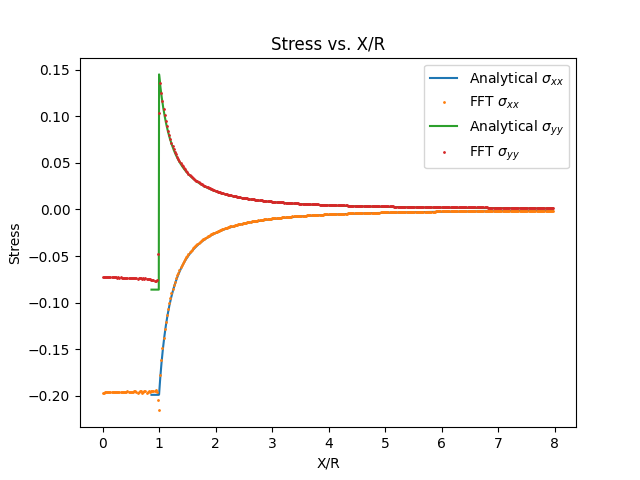
\includegraphics[width=0.45\textwidth]{images/2D_I_N_2_stress.png}}
  \hfill
  \subfigure[Error plot for in-homogeneous - normal strain - $E_p/E_m = 2$]{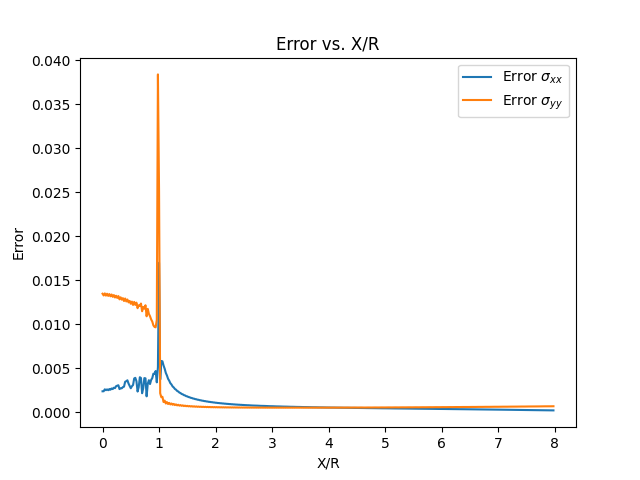
\includegraphics[width=0.45\textwidth]{images/2D_I_N_2_error.png}}
  \caption{Stress and error plots for FFT - 2D - in-homogeneous - normal strain - $E_p / E_m = 2$}
\end{figure}

\begin{table}[H]
    \centering
    \begin{tabular}{|c|c|c|}
        \hline
        &\textbf{$\sigma_{11}$} &  \textbf{$\sigma_{22}$} \\
        \hline
        $L_1$ & 0.441906 & 0.883780 \\
        \hline
        $L_2$ & 0.035345 & 0.098619 \\
        \hline 
        $L_\infty$ & 0.017003 & 0.038403 \\
        \hline
    \end{tabular}
    \caption{Error in FFT - 2D - in-homogeneous - normal strain - $E_p / E_m = 2$}
\end{table}

\paragraph{}
The input parameters, Stress profile plots, error plots, and error metrics for 2D, in-homogeneous case under normal strain conditions with $E_p / E_m = 2$ for FFT solution benchmarking are shown. Both solutions agree well except for some errors inside the inclusion. There is Low error in $\sigma_{11}$ as compared to $\sigma_{22}$, as there is a discontinuity in $\sigma_{22}$.
%%%%%%%%%%%%%%%%%%%%%%%%%%%%%%%%%%%%%%%%%%%%%%%%%%%%%%%%

\newpage
\subsubsection{In-Homogeneous Case - Normal Strain - $\frac{E_p}{E_m} = 0.5$}
\begin{table}[H]
    \centering
    \begin{tabular}{|c|c|c|}
        \hline
        & \textbf{FFT} &\textbf{Analytical}\\
        \hline
        \textbf{$a_1$} & 50 & 50 \\
        \hline
        \textbf{$a_2$} & 25 & 25 \\
        \hline
        \textbf{$\nu$} & 0.3 & 0.3 \\
        \hline
        \textbf{$E_p$} & 105 & 105 \\
        \hline
        \textbf{$E_m$} & 210 & 210 \\
        \hline
        \textbf{$\epsilon_{11}$} & 0.001 & 0.001 \\
        \hline
        \textbf{$\epsilon_{22}$} & 0.001 & 0.001 \\
        \hline
        \textbf{$\epsilon_{12}$} & 0 & 0 \\
        \hline
        \textbf{Other} & Grid size = 1024*1024, Cell size = 1*1 &  \\
        \hline
    \end{tabular}
    \caption{Input parameters for FFT - 2D - in-homogeneous - normal strain - $E_p / E_m = 0.5$}
\end{table}

\begin{figure}[htbp]
  \centering
  \subfigure[Stress plot for in-homogeneous - normal strain - $E_p / E_m = 0.5$]{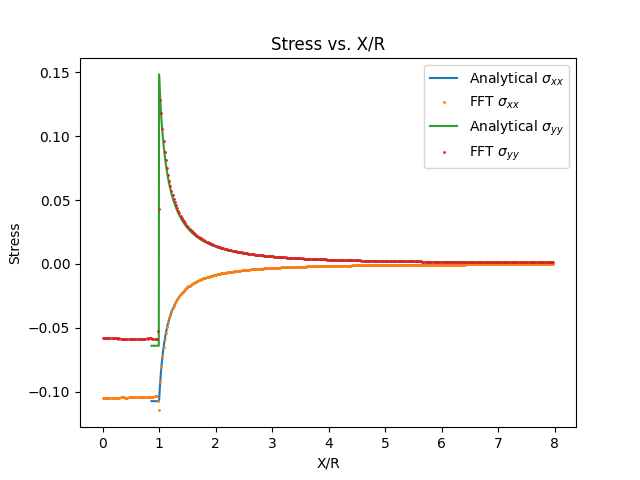
\includegraphics[width=0.45\textwidth]{images/2D_I_N_0.5_stress.png}}
  \hfill
  \subfigure[Error plot for in-homogeneous - normal strain - $E_p / E_m = 0.5$]{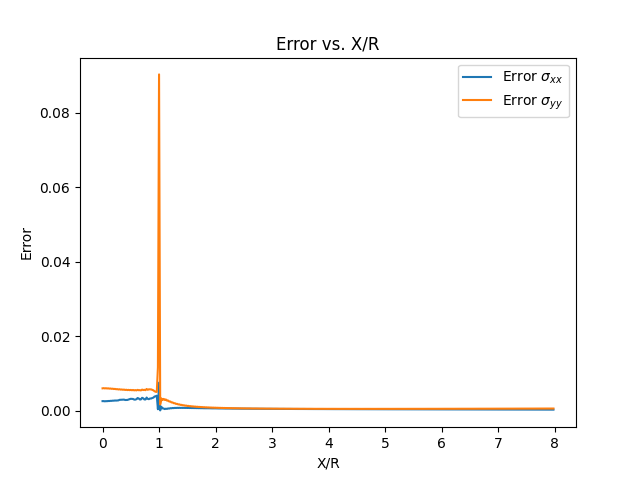
\includegraphics[width=0.45\textwidth]{images/2D_I_N_0.5_error.png}}
  \caption{Stress and error plots for FFT - 2D - in-homogeneous - normal strain - $E_p / E_m = 0.5$}
\end{figure}

\begin{table}[H]
    \centering
    \begin{tabular}{|c|c|c|}
        \hline
        &\textbf{$\sigma_{11}$} &  \textbf{$\sigma_{22}$} \\
        \hline
        $L_1$ & 0.291160 & 0.598169 \\
        \hline
        $L_2$ & 0.023594 & 0.100295 \\
        \hline 
        $L_\infty$ & 0.007504 & 0.090362 \\
        \hline
    \end{tabular}
    \caption{Error in FFT - 2D - in-homogeneous - normal strain - $E_p / E_m = 0.5$}
\end{table}

\paragraph{}
The input parameters, Stress profile plots, error plots, and error metrics for 2D, in-homogeneous case under normal strain conditions with $E_p / E_m = 0.5$ for FFT solution benchmarking are shown. Both solutions agree well except for some minimal errors inside the inclusion. There is Low error in $\sigma_{11}$ as compared to $\sigma_{22}$, as there is a discontinuity in $\sigma_{22}$.
%%%%%%%%%%%%%%%%%%%%%%%%%%%%%%%%%%%%%%%%%%%%%%%%%%%%%%%%

\newpage
\subsection{Benchmarking FFT Solution in 3D}

\subsubsection{Homogeneous Case - Normal Strain}
\begin{table}[H]
    \centering
    \begin{tabular}{|c|c|c|}
        \hline
        & \textbf{FFT} &\textbf{Analytical}\\
        \hline
        \textbf{$a_1$} & 24 & 1 \\
        \hline
        \textbf{$a_2$} & 24 & 1 \\
        \hline
        \textbf{$a_3$} & 12 & 0.5 \\
        \hline
        \textbf{$\nu$} & 0.3 & 0.3 \\
        \hline
        \textbf{$E_p$} & 210 & 210 \\
        \hline
        \textbf{$E_m$} & 210 & 210 \\
        \hline
        \textbf{$\epsilon_{11}$} & 0.001 & 0.001 \\
        \hline
        \textbf{$\epsilon_{22}$} & 0.001 & 0.001 \\
        \hline
        \textbf{$\epsilon_{33}$} & 0.001 & 0.001 \\
        \hline
        \textbf{$\epsilon_{12}, \epsilon_{23}, \epsilon_{31}$} & 0 & 0 \\
        \hline
        \textbf{Other} & Grid size = 128*128*128, Cell size = 0.4*0.4*0.4 &  \\
        \hline
    \end{tabular}
    \caption{Input parameters for FFT - 3D - homogeneous - normal strain}
\end{table}

\begin{figure}[htbp]
  \centering
  \subfigure[Stress plot for homogeneous - normal strain]{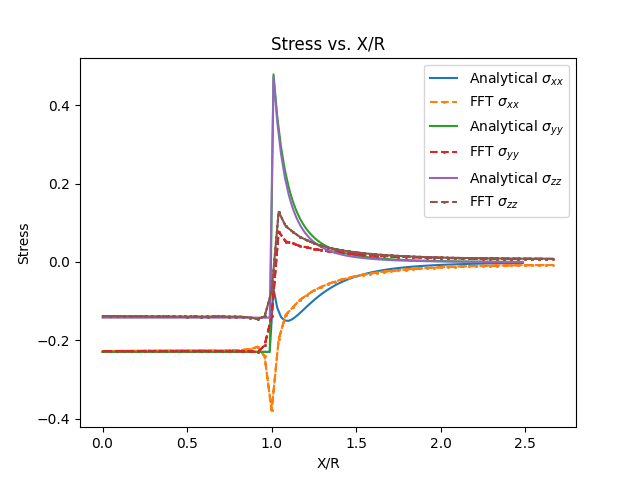
\includegraphics[width=0.45\textwidth]{images/3D_H_N_stress.png}}
  \hfill
  \subfigure[Error plot for homogeneous - normal strain]{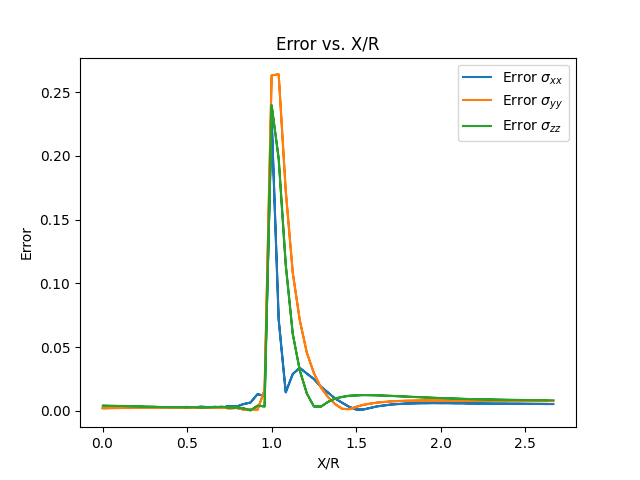
\includegraphics[width=0.45\textwidth]{images/3D_H_N_error.png}}
  \caption{Stress and error plots for FFT - 3D - homogeneous - normal strain}
\end{figure}

\begin{table}[H]
    \centering
    \begin{tabular}{|c|c|c|c|}
        \hline
        &\textbf{$\sigma_{11}$} &  \textbf{$\sigma_{22}$} & \textbf{$\sigma_{33}$}\\
        \hline
        $L_1$ & 1.442848 & 2.536335 & 2.119077 \\
        \hline
        $L_2$ & 0.356524 & 0.618075 & 0.486176 \\
        \hline 
        $L_\infty$ & 0.229643 & 0.263992 & 0.239790 \\
        \hline
    \end{tabular}
    \caption{Error in FFT - 3D - homogeneous - normal strain}
\end{table}  

\paragraph{}
The input parameters, Stress profile plots, error plots, and error metrics for 3D, homogeneous case under normal strain conditions for FFT solution benchmarking are shown. Both solutions agree well inside inclusion and far away from inclusion. There is considerable error at the boundary, which can be seen from the error plot.
%%%%%%%%%%%%%%%%%%%%%%%%%%%%%%%%%%%%%%%%%%%%%%%%%%%%%%%%%%%%%%%

\newpage

\subsubsection{In-Homogeneous Case - Normal Strain - $E_p/E_m = 2$}
\begin{table}[H]
    \centering
    \begin{tabular}{|c|c|c|}
        \hline
        & \textbf{FFT} &\textbf{Analytical}\\
        \hline
        \textbf{$a_1$} & 24 & 1 \\
        \hline
        \textbf{$a_2$} & 24 & 1 \\
        \hline
        \textbf{$a_3$} & 12 & 0.5 \\
        \hline
        \textbf{$\nu$} & 0.3 & 0.3 \\
        \hline
        \textbf{$E_p$} & 420 & 420 \\
        \hline
        \textbf{$E_m$} & 210 & 210 \\
        \hline
        \textbf{$\epsilon_{11}$} & 0.001 & 0.001 \\
        \hline
        \textbf{$\epsilon_{22}$} & 0.001 & 0.001 \\
        \hline
        \textbf{$\epsilon_{33}$} & 0.001 & 0.001 \\
        \hline
        \textbf{$\epsilon_{12}, \epsilon_{23}, \epsilon_{31}$} & 0 & 0 \\
        \hline
        \textbf{Other} & Grid size = 128*128*128, Cell size = 0.4*0.4*0.4 &  \\
        \hline
    \end{tabular}
    \caption{Input parameters for FFT - 3D - in-homogeneous - normal strain - $E_p/E_m = 2$}
\end{table}

\begin{figure}[htbp]
  \centering
  \subfigure[Stress plot for in-homogeneous - normal strain - $E_p/E_m = 2$]{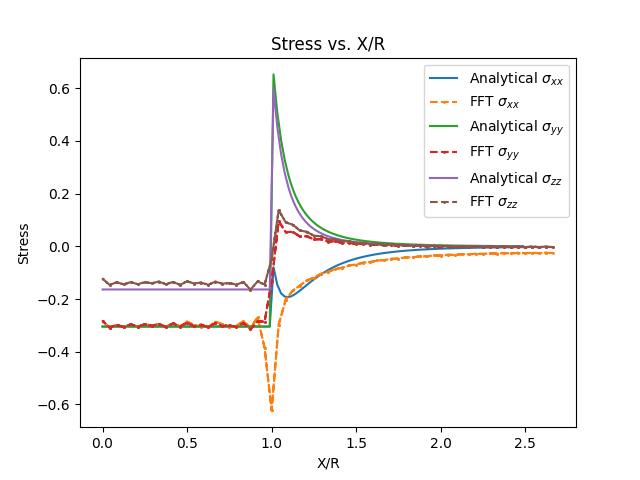
\includegraphics[width=0.45\textwidth]{images/3D_I_N_2_stress.png}}
  \hfill
  \subfigure[Error plot for in-homogeneous - normal strain - $E_p/E_m = 2$]{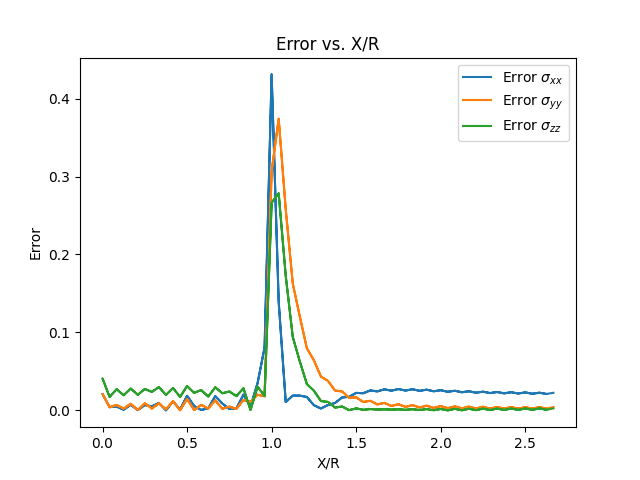
\includegraphics[width=0.45\textwidth]{images/3D_I_N_2_error.png}}
  \caption{Stress and error plots for FFT - 3D - in-homogeneous - normal strain - $E_p/E_m = 2$}
\end{figure}

\begin{table}[H]
    \centering
    \begin{tabular}{|c|c|c|c|}
        \hline
        &\textbf{$\sigma_{11}$} &  \textbf{$\sigma_{22}$} & \textbf{$\sigma_{33}$}\\
        \hline
        $L_1$ & 3.291609 & 3.690918 & 3.108819 \\
        \hline
        $L_2$ & 0.683009 & 0.848983 & 0.644062 \\
        \hline 
        $L_\infty$ & 0.430938 & 0.374037 & 0.278481 \\
        \hline
    \end{tabular}
    \caption{Error in FFT - 3D - in-homogeneous - normal strain - $E_p/E_m = 2$}
\end{table}

\paragraph{}
The input parameters, Stress profile plots, error plots, and error metrics for 3D, in-homogeneous case under normal strain conditions with $E_p / E_m = 2$ for FFT solution benchmarking are shown. Both solutions agree well inside and far-away from inclusion. The oscillatory behavior of the FFT solution can be seen from the stress plot. Stress profiles have a huge error around the boundary of the inclusion.
%%%%%%%%%%%%%%%%%%%%%%%%%%%%%%%%%%%%%%%%%%%%%%%%%%%%%%%%%%%%%%%

\newpage

\subsubsection{In-Homogeneous Case - Normal Strain - $E_p/E_m = 0.5$}
\begin{table}[H]
    \centering
    \begin{tabular}{|c|c|c|}
        \hline
        & \textbf{FFT} &\textbf{Analytical}\\
        \hline
        \textbf{$a_1$} & 24 & 1 \\
        \hline
        \textbf{$a_2$} & 24 & 1 \\
        \hline
        \textbf{$a_3$} & 12 & 0.5 \\
        \hline
        \textbf{$\nu$} & 0.3 & 0.3 \\
        \hline
        \textbf{$E_p$} & 105 & 105 \\
        \hline
        \textbf{$E_m$} & 210 & 210 \\
        \hline
        \textbf{$\epsilon_{11}$} & 0.001 & 0.001 \\
        \hline
        \textbf{$\epsilon_{22}$} & 0.001 & 0.001 \\
        \hline
        \textbf{$\epsilon_{33}$} & 0.001 & 0.001 \\
        \hline
        \textbf{$\epsilon_{12}, \epsilon_{23}, \epsilon_{31}$} & 0 & 0 \\
        \hline
        \textbf{Other} & Grid size = 128*128*128, Cell size = 0.4*0.4*0.4 &  \\
        \hline
    \end{tabular}
    \caption{Input parameters for FFT - 3D - in-homogeneous - normal strain - $E_p/E_m = 0.5$}
\end{table}

\begin{figure}[htbp]
  \centering
  \subfigure[Stress plot for in-homogeneous - normal strain - $E_p/E_m = 0.5$]{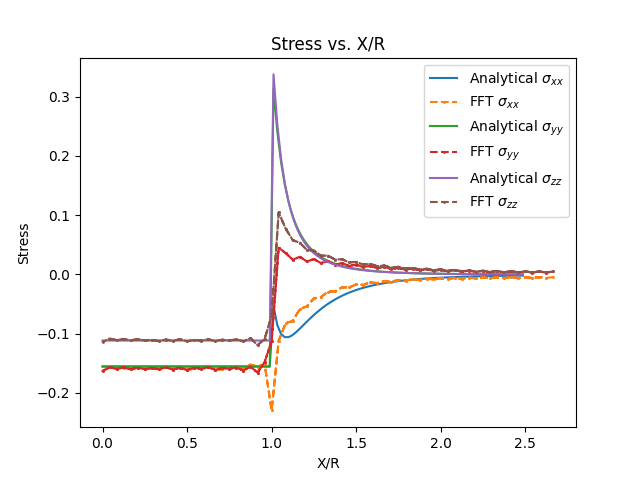
\includegraphics[width=0.45\textwidth]{images/3D_I_N_0.5_stress.png}}
  \hfill
  \subfigure[Error plot for in-homogeneous - normal strain - $E_p/E_m = 0.5$]{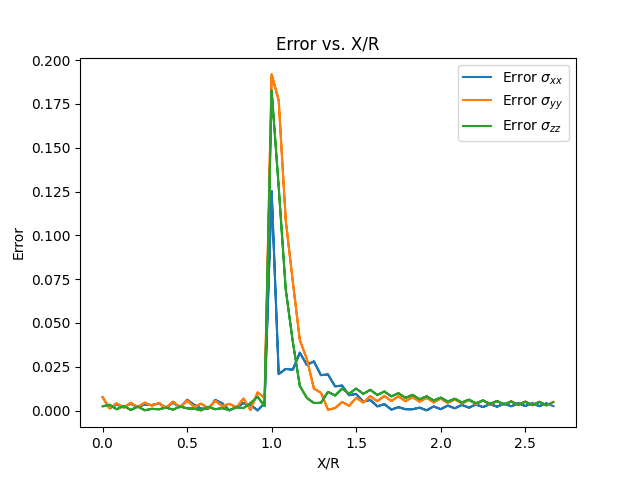
\includegraphics[width=0.45\textwidth]{images/3D_I_N_0.5_error.png}}
  \caption{Stress and error plots for FFT - 3D - in-homogeneous - normal strain - $E_p/E_m = 0.5$}
\end{figure}

\begin{table}[H]
    \centering
    \begin{tabular}{|c|c|c|c|}
        \hline
        &\textbf{$\sigma_{11}$} &  \textbf{$\sigma_{22}$} & \textbf{$\sigma_{33}$}\\
        \hline
        $L_1$ & 1.019671 & 1.793256 & 1.442135 \\
        \hline
        $L_2$ & 0.208362 & 0.423241 & 0.341527 \\
        \hline 
        $L_\infty$ & 0.125253 & 0.191841 & 0.182675 \\
        \hline
    \end{tabular}
    \caption{Error in FFT - 3D - in-homogeneous - normal strain - $E_p/E_m = 0.5$}
\end{table}

\paragraph{}
The input parameters, Stress profile plots, error plots, and error metrics for 3D, in-homogeneous case under normal strain conditions with $E_p / E_m = 0.5$ for FFT solution benchmarking are shown. Both solutions agree well inside and far-away from inclusion. The oscillatory behavior of the FFT solution can be seen from the stress plot. Stress profiles have a huge error around the boundary of the inclusion.
%%%%%%%%%%%%%%%%%%%%%%%%%%%%%%%%%%%%%%%%%%%%%%%%%%%%%%%%%%%%%%%

\newpage
\subsection{Benchmarking Alamo Solution in 2D}

\subsubsection{Homogeneous Case - Normal Strain}
\begin{table}[H]
    \centering
    \begin{tabular}{|c|c|c|}
        \hline
        & \textbf{Alamo} &\textbf{Analytical}\\
        \hline
        \textbf{$a_1$} & 1 & 1 \\
        \hline
        \textbf{$a_2$} & 0.5 & 0.5 \\
        \hline
        \textbf{$\nu$} & 0.3 & 0.3 \\
        \hline
        \textbf{$E_p$} & 210 & 210 \\
        \hline
        \textbf{$E_m$} & 210 & 210 \\
        \hline
        \textbf{$\epsilon_{11}$} & 0.001 & 0.001 \\
        \hline
        \textbf{$\epsilon_{22}$} & 0.001 & 0.001 \\
        \hline
        \textbf{$\epsilon_{12}$} & 0 & 0 \\
        \hline
        \textbf{Other} & Grid size = 1024*1024, diffuse boundary = 0.1&  \\
        \hline
    \end{tabular}
    \caption{Input parameters for alamo - 2D - homogeneous - normal strain}
\end{table}

\begin{figure}[htbp]
  \centering
  \subfigure[Stress plot for homogeneous - normal strain]{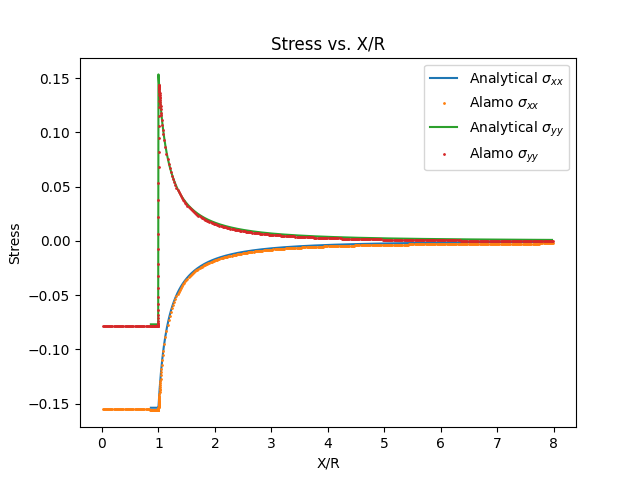
\includegraphics[width=0.45\textwidth]{images/2D_A_H_N_stress.png}}
  \hfill
  \subfigure[Error plot for homogeneous - normal strain]{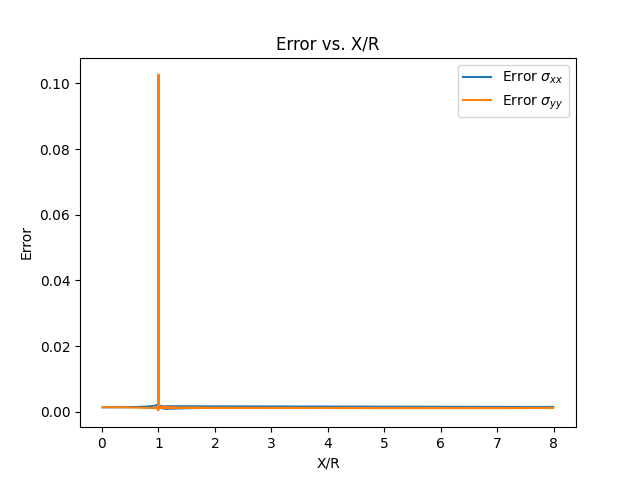
\includegraphics[width=0.45\textwidth]{images/2D_A_H_N_error.png}}
  \caption{Stress and error plots for Alamo - 2D - homogeneous - normal strain}
\end{figure}

\begin{table}[H]
    \centering
    \begin{tabular}{|c|c|c|}
        \hline
        &\textbf{$\sigma_{11}$} &  \textbf{$\sigma_{22}$} \\
        \hline
        $L_1$ & 0.659354 & 1.495967 \\
        \hline
        $L_2$ & 0.030559 & 0.251939  \\
        \hline 
        $L_\infty$ & 0.002471 & 0.102727 \\
        \hline
    \end{tabular}
    \caption{Error in Alamo - 2D - homogeneous - normal strain}
\end{table}

\paragraph{}
The input parameters, Stress profile plots, error plots, and error metrics for 2D, homogeneous case under normal strain conditions for Alamo solution benchmarking are shown. Both solutions agree well in the entire range of the x-axis, except for an error at the discontinuity near the boundary of the inclusion.

%%%%%%%%%%%%%%%%%%%%%%%%%%%%%%%%%%%%%%%%%%%%%%%%%

\newpage

\subsubsection{Homogeneous Case - Shear Strain}
\begin{table}[H]
    \centering
    \begin{tabular}{|c|c|c|}
        \hline
        & \textbf{Alamo} &\textbf{Analytical}\\
        \hline
        \textbf{$a_1$} & 1 & 1 \\
        \hline
        \textbf{$a_2$} & 0.5 & 0.5 \\
        \hline
        \textbf{$\nu$} & 0.3 & 0.3 \\
        \hline
        \textbf{$E_p$} & 210 & 210 \\
        \hline
        \textbf{$E_m$} & 210 & 210 \\
        \hline
        \textbf{$\epsilon_{11}$} & 0 & 0 \\
        \hline
        \textbf{$\epsilon_{22}$} & 0 & 0 \\
        \hline
        \textbf{$\epsilon_{12}$} & 0.001 & 0.001 \\
        \hline
        \textbf{Other} & Grid size = 1024*1024, diffuse boundary = 0.1&  \\
        \hline
    \end{tabular}
    \caption{Input parameters for Alamo - 2D - homogeneous - shear strain}
\end{table}

\begin{figure}[htbp]
  \centering
  \subfigure[Stress plot for homogeneous - shear strain]{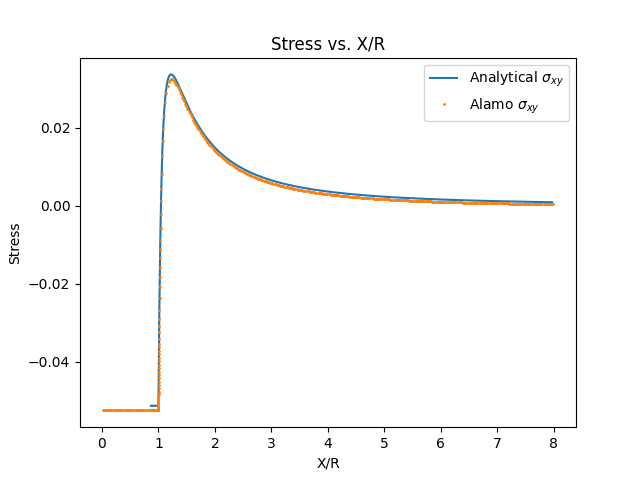
\includegraphics[width=0.45\textwidth]{images/2D_A_H_S_stress.png}}
  \hfill
  \subfigure[Error plot for homogeneous - shear strain]{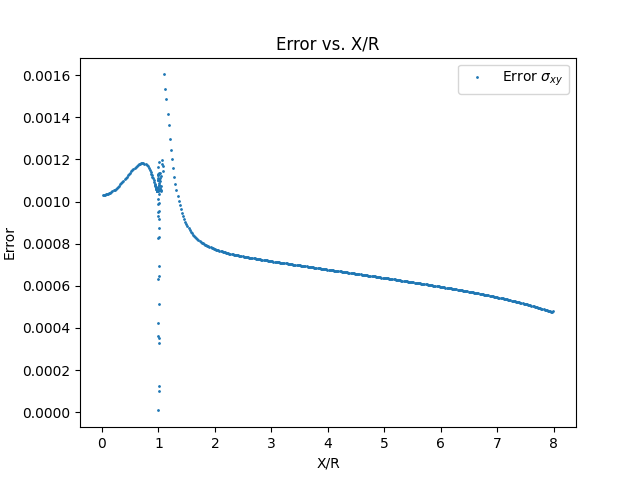
\includegraphics[width=0.45\textwidth]{images/2D_A_H_S_error.png}}
  \caption{Stress and error plots for Alamo - 2D - homogeneous - shear strain}
\end{figure}

\begin{table}[H]
    \centering
    \begin{tabular}{|c|c|c|}
        \hline
        &\textbf{$\sigma_{12}$} \\
        \hline
        $L_1$ & 0.370328 \\
        \hline
        $L_2$ & 0.017624 \\
        \hline 
        $L_\infty$ & 0.001603 \\
        \hline
    \end{tabular}
    \caption{Error in Alamo - 2D - homogeneous - shear strain}
\end{table}

\paragraph{}
The input parameters, stress profile plots, error plots, and error metrics for 2D, homogeneous case under shear strain conditions for Alamo solution benchmarking are shown. Both solutions agree well in the entire range of the x-axis, with minimal errors throughout the range on the x-axis. The minimal nature of the error can be observed from the range on the y-axis of the error plot.

%%%%%%%%%%%%%%%%%%%%%%%%%%%%%%%%%%%%%%%%%%%%%%%%%

\newpage

\subsubsection{In-Homogeneous Case - Normal Strain - $E_p/E_m = 2$}
\begin{table}[H]
    \centering
    \begin{tabular}{|c|c|c|}
        \hline
        & \textbf{Alamo} &\textbf{Analytical}\\
        \hline
        \textbf{$a_1$} & 1 & 1 \\
        \hline
        \textbf{$a_2$} & 0.5 & 0.5 \\
        \hline
        \textbf{$\nu$} & 0.3 & 0.3 \\
        \hline
        \textbf{$E_p$} & 420 & 420 \\
        \hline
        \textbf{$E_m$} & 210 & 210 \\
        \hline
        \textbf{$\epsilon_{11}$} & 0.001 & 0.001 \\
        \hline
        \textbf{$\epsilon_{22}$} & 0.001 & 0.001 \\
        \hline
        \textbf{$\epsilon_{12}$} & 0 & 0 \\
        \hline
        \textbf{Other} & Grid size = 1024*1024, diffuse boundary = 0.1&  \\
        \hline
    \end{tabular}
    \caption{Input parameters for Alamo - 2D - in-homogeneous - normal strain - $E_p/E_m = 2$}
\end{table}

\begin{figure}[htbp]
  \centering
  \subfigure[Stress plot for in-homogeneous - normal strain - $E_p/E_m = 2$]{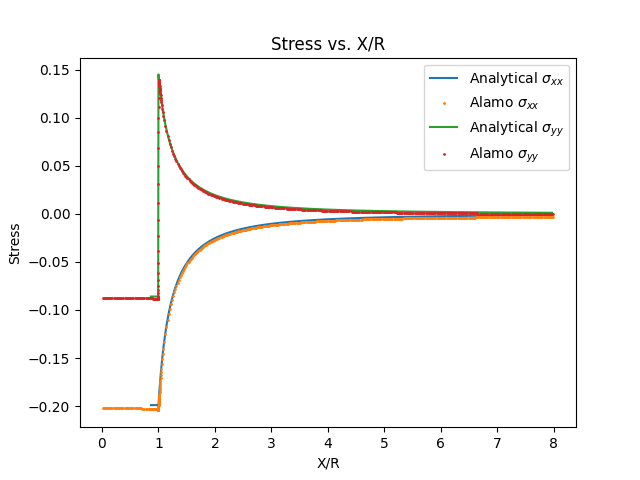
\includegraphics[width=0.45\textwidth]{images/2D_A_I_N_2_stress.png}}
  \hfill
  \subfigure[Error plot for in-homogeneous - normal strain - $E_p/E_m = 2$]{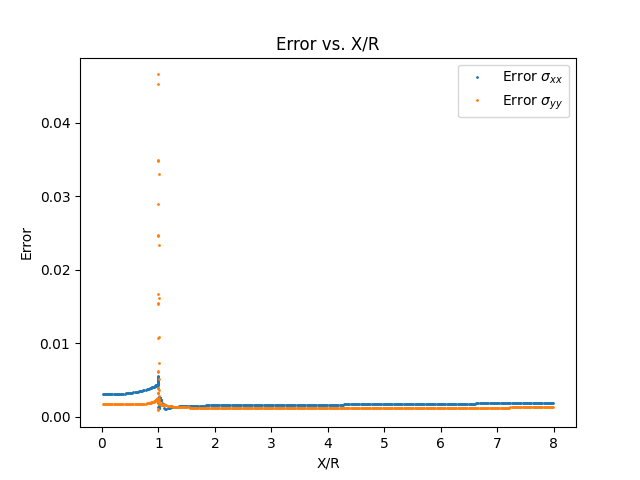
\includegraphics[width=0.45\textwidth]{images/2D_A_I_N_2_error.png}}
  \caption{Stress and error plots for alamo - 2D - in-homogeneous - normal strain - $E_p/E_m = 2$}
\end{figure}

\begin{table}[H]
    \centering
    \begin{tabular}{|c|c|c|}
        \hline
        &\textbf{$\sigma_{11}$} &  \textbf{$\sigma_{22}$} \\
        \hline
        $L_1$ & 1.021290 & 1.056446 \\
        \hline
        $L_2$ & 0.050688 & 0.112844  \\
        \hline 
        $L_\infty$ & 0.005488 & 0.046580 \\
        \hline
    \end{tabular}
    \caption{Error in Alamo - 2D - in-homogeneous - normal strain - $E_p/E_m = 2$}
\end{table}

\paragraph{}
The input parameters, stress profile plots, error plots, and error metrics for 2D, in-homogeneous case under normal strain conditions with $E_p/E_m = 2$ for Alamo solution benchmarking are shown. Both solutions agree well in the entire range of the x-axis, with considerable errors inside the inclusion and negligible errors outside the inclusion. The error profile shows a spike in error at the boundary of inclusion.

%%%%%%%%%%%%%%%%%%%%%%%%%%%%%%%%%%%%%%%%%%%%%%%%%
\newpage

\subsubsection{In-Homogeneous Case - Shear Strain - $E_p/E_m = 2$}
\begin{table}[H]
    \centering
    \begin{tabular}{|c|c|c|}
        \hline
        & \textbf{Alamo} &\textbf{Analytical}\\
        \hline
        \textbf{$a_1$} & 1 & 1 \\
        \hline
        \textbf{$a_2$} & 0.5 & 0.5 \\
        \hline
        \textbf{$\nu$} & 0.3 & 0.3 \\
        \hline
        \textbf{$E_p$} & 420 & 420 \\
        \hline
        \textbf{$E_m$} & 210 & 210 \\
        \hline
        \textbf{$\epsilon_{11}$} & 0 & 0 \\
        \hline
        \textbf{$\epsilon_{22}$} & 0 & 0 \\
        \hline
        \textbf{$\epsilon_{12}$} & 0.001 & 0.001 \\
        \hline
        \textbf{Other} & Grid size = 1024*1024, diffuse boundary = 0.1&  \\
        \hline
    \end{tabular}
    \caption{Input parameters for Alamo - 2D - in-homogeneous - shear strain - $E_p/E_m = 2$}
\end{table}

\begin{figure}[htbp]
  \centering
  \subfigure[Stress plot for in-homogeneous - shear strain - $E_p/E_m = 2$]{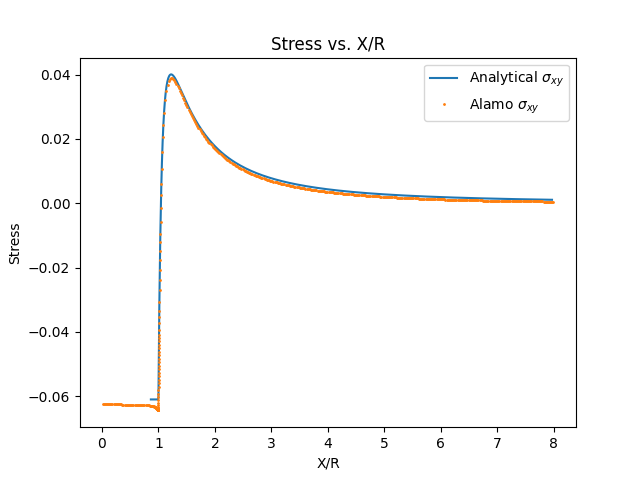
\includegraphics[width=0.45\textwidth]{images/2D_A_I_S_2_stress.png}}
  \hfill
  \subfigure[Error plot for in-homogeneous - shear strain - $E_p/E_m = 2$]{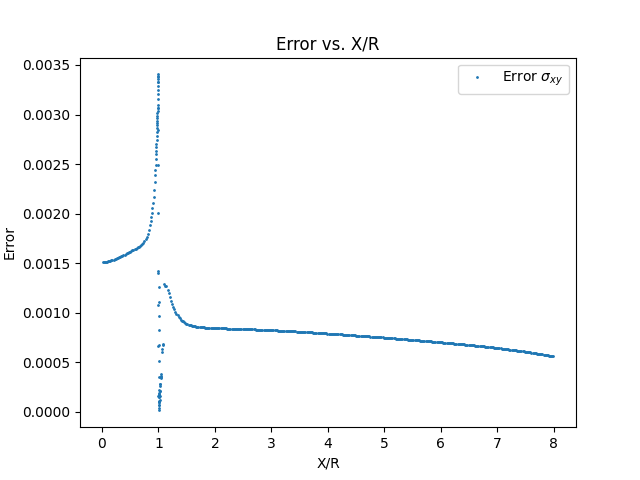
\includegraphics[width=0.45\textwidth]{images/2D_A_I_S_2_error.png}}
  \caption{Stress and error plots for Alamo - 2D - in-homogeneous - shear strain - $E_p/E_m = 2$}
\end{figure}

\begin{table}[H]
    \centering
    \begin{tabular}{|c|c|c|}
        \hline
        &\textbf{$\sigma_{12}$} \\
        \hline
        $L_1$ & 0.478343 \\
        \hline
        $L_2$ & 0.026029  \\
        \hline 
        $L_\infty$ & 0.003405\\
        \hline
    \end{tabular}
    \caption{Error in Alamo - 2D - in-homogeneous - shear strain - $E_p/E_m = 2$}
\end{table}

\paragraph{}
The input parameters, stress profile plots, error plots, and error metrics for 2D, in-homogeneous case under shear strain conditions with $E_p/E_m = 2$ for Alamo solution benchmarking are shown. Both solutions agree well in the entire range of the x-axis. The minimal nature of the error can be noticed by observing the scale on the y-axis of the error plot. There is also a spike in error at the inclusion boundary.

%%%%%%%%%%%%%%%%%%%%%%%%%%%%%%%%%%%%%%%%%%%%%%%%%
\newpage

\subsubsection{In-Homogeneous Case - Normal Strain - $E_p/E_m = 0.5$}
\begin{table}[H]
    \centering
    \begin{tabular}{|c|c|c|}
        \hline
        & \textbf{Alamo} &\textbf{Analytical}\\
        \hline
        \textbf{$a_1$} & 1 & 1 \\
        \hline
        \textbf{$a_2$} & 0.5 & 0.5 \\
        \hline
        \textbf{$\nu$} & 0.3 & 0.3 \\
        \hline
        \textbf{$E_p$} & 105 & 105 \\
        \hline
        \textbf{$E_m$} & 210 & 210 \\
        \hline
        \textbf{$\epsilon_{11}$} & 0.001 & 0.001 \\
        \hline
        \textbf{$\epsilon_{22}$} & 0.001 & 0.001 \\
        \hline
        \textbf{$\epsilon_{12}$} & 0 & 0 \\
        \hline
        \textbf{Other} & Grid size = 1024*1024, diffuse boundary = 0.1&  \\
        \hline
    \end{tabular}
    \caption{Input parameters for Alamo - 2D - in-homogeneous - normal strain - $E_p/E_m = 0.5$}
\end{table}

\begin{figure}[htbp]
  \centering
  \subfigure[Stress plot for in-homogeneous - normal strain - $E_p/E_m = 0.5$]{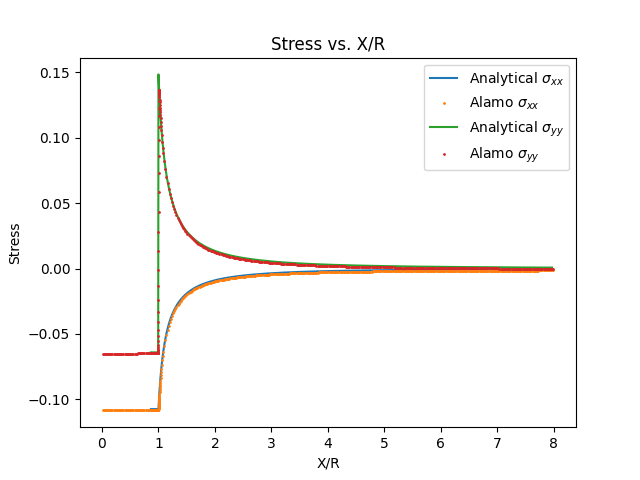
\includegraphics[width=0.45\textwidth]{images/2D_A_I_N_0.5_stress.png}}
  \hfill
  \subfigure[Error plot for in-homogeneous - normal strain - $E_p/E_m = 0.5$]{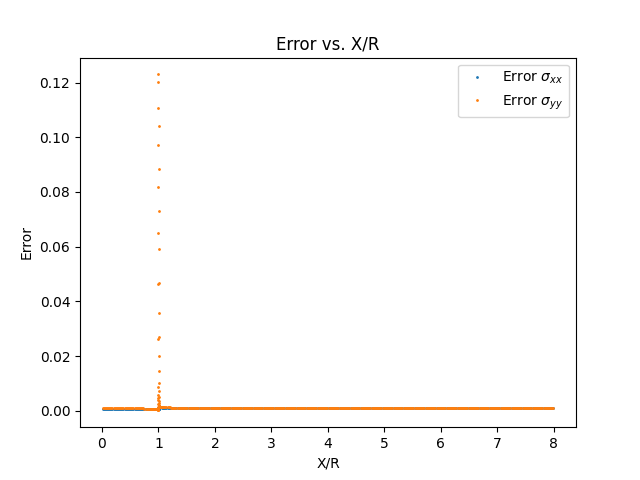
\includegraphics[width=0.45\textwidth]{images/2D_A_I_N_0.5_error.png}}
  \caption{Stress and error plots for Alamo - 2D - in-homogeneous - normal strain - $E_p/E_m = 0.5$}
\end{figure}

\begin{table}[H]
    \centering
    \begin{tabular}{|c|c|c|}
        \hline
        &\textbf{$\sigma_{11}$} &  \textbf{$\sigma_{22}$} \\
        \hline
        $L_1$ & 0.429350 & 1.626370 \\
        \hline
        $L_2$ & 0.019952 & 0.313113  \\
        \hline 
        $L_\infty$ & 0.001567 & 0.123013 \\
        \hline
    \end{tabular}
    \caption{Error in Alamo - 2D - in-homogeneous - normal strain - $E_p/E_m = 0.5$}
\end{table}


\paragraph{}
The input parameters, stress profile plots, error plots, and error metrics for 2D, in-homogeneous case under normal strain conditions with $E_p/E_m = 0.5$ for Alamo solution benchmarking are shown. Both solutions agree well in the entire range of the x-axis. There is also a spike in error at the inclusion boundary.

%%%%%%%%%%%%%%%%%%%%%%%%%%%%%%%%%%%%%%%%%%%%%%%%%
\newpage

\subsubsection{In-Homogeneous Case - Shear Strain - $E_p/E_m = 0.5$}
\begin{table}[H]
    \centering
    \begin{tabular}{|c|c|c|}
        \hline
        & \textbf{Alamo} &\textbf{Analytical}\\
        \hline
        \textbf{$a_1$} & 1 & 1 \\
        \hline
        \textbf{$a_2$} & 0.5 & 0.5 \\
        \hline
        \textbf{$\nu$} & 0.3 & 0.3 \\
        \hline
        \textbf{$E_p$} & 105 & 105 \\
        \hline
        \textbf{$E_m$} & 210 & 210 \\
        \hline
        \textbf{$\epsilon_{11}$} & 0 & 0 \\
        \hline
        \textbf{$\epsilon_{22}$} & 0 & 0 \\
        \hline
        \textbf{$\epsilon_{12}$} & 0.001 & 0.001 \\
        \hline
        \textbf{Other} & Grid size = 1024*1024, diffuse boundary = 0.1&  \\
        \hline
    \end{tabular}
    \caption{Input parameters for Alamo - 2D - in-homogeneous - shear strain - $E_p/E_m = 0.5$}
\end{table}

\begin{figure}[htbp]
  \centering
  \subfigure[Stress plot for in-homogeneous - shear strain - $E_p/E_m = 0.5$]{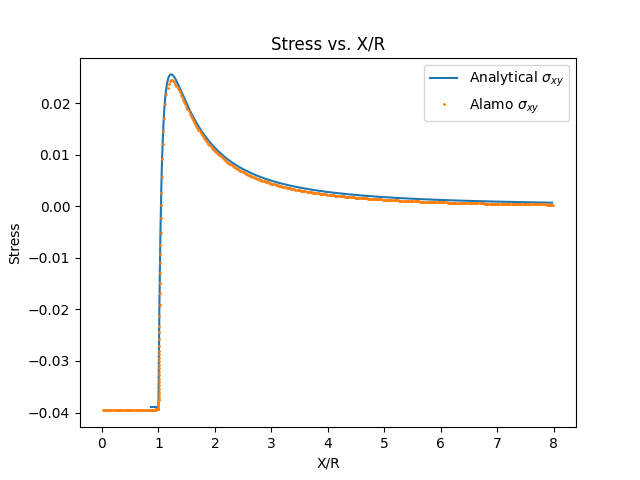
\includegraphics[width=0.45\textwidth]{images/2D_A_I_S_0.5_stress.png}}
  \hfill
  \subfigure[Error plot for in-homogeneous - shear strain - $E_p/E_m = 0.5$]{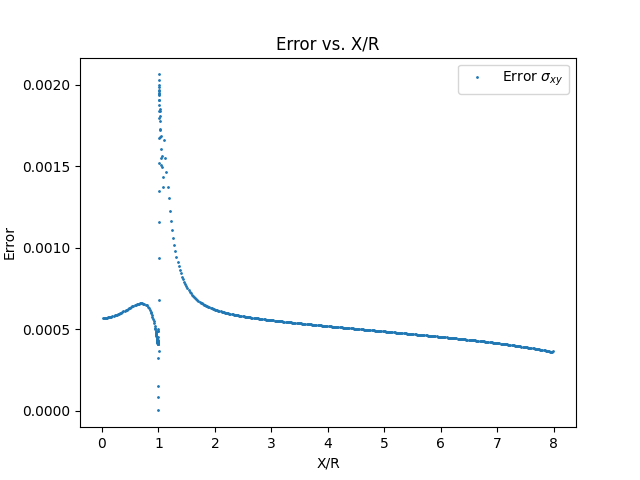
\includegraphics[width=0.45\textwidth]{images/2D_A_I_S_0.5_error.png}}
  \caption{Stress and error plots for Alamo - 2D - in-homogeneous - shear strain - $E_p/E_m = 0.5$}
\end{figure}

\begin{table}[H]
    \centering
    \begin{tabular}{|c|c|c|}
        \hline
        &\textbf{$\sigma_{12}$} \\
        \hline
        $L_1$ & 0.296722 \\
        \hline
        $L_2$ & 0.015518  \\
        \hline 
        $L_\infty$ & 0.002065 \\
        \hline
    \end{tabular}
    \caption{Error in Alamo - 2D - in-homogeneous - shear strain - $E_p/E_m = 0.5$}
\end{table}

\paragraph{}
The input parameters, stress profile plots, error plots, and error metrics for 2D, in-homogeneous case under shear strain conditions with $E_p/E_m = 0.5$ for Alamo solution benchmarking are shown. Both solutions agree well in the entire range of the x-axis. The minimal nature of the error can be noticed by observing the scale on the y-axis of the error plot. There is also a spike in error at the inclusion boundary.

%%%%%%%%%%%%%%%%%%%%%%%%%%%%%%%%%%%%%%%%%%%%%%%%%
\newpage
\subsection{Benchmarking Alamo Solution in 3D}

\subsubsection{Homogeneous Case - Normal Strain}
\begin{table}[H]
    \centering
    \begin{tabular}{|c|c|c|}
        \hline
        & \textbf{Alamo} &\textbf{Analytical}\\
        \hline
        \textbf{$a_1$} & 1 & 1 \\
        \hline
        \textbf{$a_2$} & 1 & 1 \\
        \hline
        \textbf{$a_3$} & 0.5 & 0.5 \\
        \hline
        \textbf{$\nu$} & 0.3 & 0.3 \\
        \hline
        \textbf{$E_p$} & 210 & 210 \\
        \hline
        \textbf{$E_m$} & 210 & 210 \\
        \hline
        \textbf{$\epsilon_{11}$} & 0.001 & 0.001 \\
        \hline
        \textbf{$\epsilon_{22}$} & 0.001 & 0.001 \\
        \hline
        \textbf{$\epsilon_{33}$} & 0.001 & 0.001 \\
        \hline
        \textbf{$\epsilon_{12}, \epsilon_{23}, \epsilon_{31}$} & 0 & 0 \\
        \hline
        \textbf{Other} & Grid size = 32*32*32, diffuse boundary = 0.1 &  \\
        \hline
    \end{tabular}
    \caption{Input parameters for Alamo - 3D - homogeneous - normal strain}
\end{table}

\begin{figure}[htbp]
  \centering
  \subfigure[Stress plot for homogeneous - normal strain]{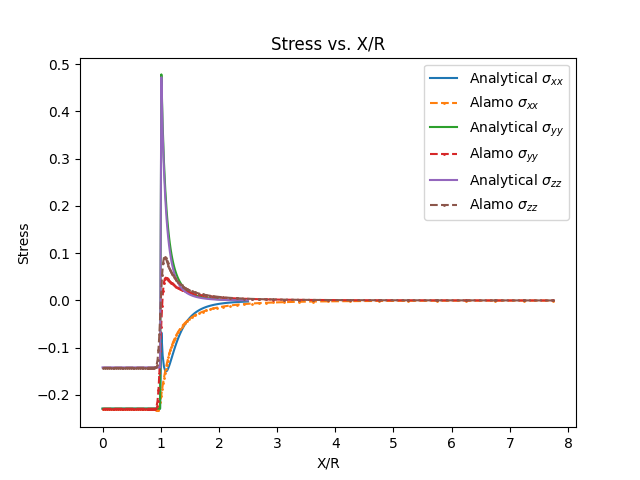
\includegraphics[width=0.45\textwidth]{images/3D_A_H_N_stress.png}}
  \hfill
  \subfigure[Error plot for homogeneous - normal strain]{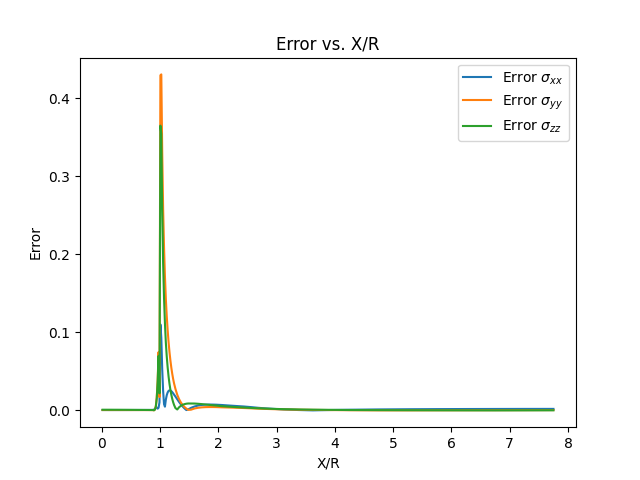
\includegraphics[width=0.45\textwidth]{images/3D_A_H_N_error.png}}
  \caption{Stress and error plots for Alamo - 3D - homogeneous - normal strain}
\end{figure}

\begin{table}[H]
    \centering
    \begin{tabular}{|c|c|c|c|}
        \hline
        &\textbf{$\sigma_{11}$} &  \textbf{$\sigma_{22}$} & \textbf{$\sigma_{33}$}\\
        \hline
        $L_1$ & 0.722275 & 2.908479 & 2.103092 \\
        \hline
        $L_2$ & 0.175746 & 0.836623 & 0.649355 \\
        \hline 
        $L_\infty$ & 0.110245 & 0.430738 & 0.365048 \\
        \hline
    \end{tabular}
    \caption{Error in Alamo - 3D - homogeneous - normal strain}
\end{table}

\paragraph{}
The input parameters, stress profile plots, error plots, and error metrics for 3D, homogeneous case under normal strain conditions for Alamo solution benchmarking are shown. Both solutions agree well in the entire range of the x-axis. There is a spike in error at the inclusion boundary.
%%%%%%%%%%%%%%%%%%%%%%%%%%%%%%%%%%%%%%%%%%%%%%%%%%%%%%%%%%%%%%%

\newpage

\subsubsection{Homogeneous Case - Shear Strain}
\begin{table}[H]
    \centering
    \begin{tabular}{|c|c|c|}
        \hline
        & \textbf{Alamo} &\textbf{Analytical}\\
        \hline
        \textbf{$a_1$} & 1 & 1 \\
        \hline
        \textbf{$a_2$} & 1 & 1 \\
        \hline
        \textbf{$a_3$} & 0.5 & 0.5 \\
        \hline
        \textbf{$\nu$} & 0.3 & 0.3 \\
        \hline
        \textbf{$E_p$} & 210 & 210 \\
        \hline
        \textbf{$E_m$} & 210 & 210 \\
        \hline
        \textbf{$\epsilon_{11}$} & 0 & 0 \\
        \hline
        \textbf{$\epsilon_{22}$} & 0 & 0 \\
        \hline
        \textbf{$\epsilon_{33}$} & 0 & 0 \\
        \hline
        \textbf{$\epsilon_{12}, \epsilon_{23}, \epsilon_{31}$} & 0.001 & 0.001 \\
        \hline
        \textbf{Other} & Grid size = 32*32*32, diffuse boundary = 0.1 &  \\
        \hline
    \end{tabular}
    \caption{Input parameters for Alamo - 3D - homogeneous - shear strain}
\end{table}

\begin{figure}[htbp]
  \centering
  \subfigure[Stress plot for homogeneous - shear strain]{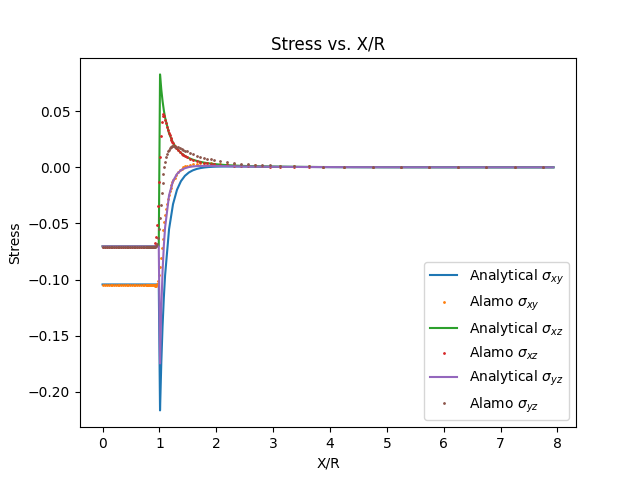
\includegraphics[width=0.45\textwidth]{images/3D_A_H_S_stress.png}}
  \hfill
  \subfigure[Error plot for homogeneous - shear strain]{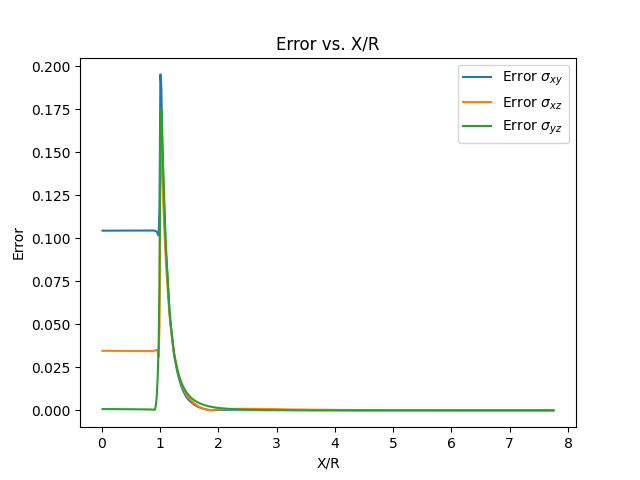
\includegraphics[width=0.45\textwidth]{images/3D_A_H_S_error.png}}
  \caption{Stress and error plots for Alamo - 3D - homogeneous - shear strain}
\end{figure}

\begin{table}[H]
    \centering
    \begin{tabular}{|c|c|c|c|}
        \hline
        &\textbf{$\sigma_{12}$} &  \textbf{$\sigma_{23}$} & \textbf{$\sigma_{13}$}\\
        \hline
        $L_1$ & 5.820405 & 1.801642 & 2.882413 \\
        \hline
        $L_2$ & 0.789585 & 0.424529 & 0.433724 \\
        \hline 
        $L_\infty$ & 0.195187 & 0.175271 & 0.155894 \\
        \hline
    \end{tabular}
    \caption{Error in Alamo - 3D - homogeneous - shear strain}
\end{table}
\paragraph{}
The input parameters, stress profile plots, error plots, and error metrics for 3D, homogeneous case under shear strain conditions for Alamo solution benchmarking are shown. Both solutions agree well outside the inclusion. There are discrete error levels inside the inclusion, which leads to an increase in error metrics. There is also a spike in error at the inclusion boundary.
%%%%%%%%%%%%%%%%%%%%%%%%%%%%%%%%%%%%%%%%%%%%%%%%%%%%%%%%%%%%%%%

\newpage

\subsubsection{In-Homogeneous Case - Normal Strain - $E_p/E_m = 2$}
\begin{table}[H]
    \centering
    \begin{tabular}{|c|c|c|}
        \hline
        & \textbf{Alamo} &\textbf{Analytical}\\
        \hline
        \textbf{$a_1$} & 1 & 1 \\
        \hline
        \textbf{$a_2$} & 1 & 1 \\
        \hline
        \textbf{$a_3$} & 0.5 & 0.5 \\
        \hline
        \textbf{$\nu$} & 0.3 & 0.3 \\
        \hline
        \textbf{$E_p$} & 420 & 420 \\
        \hline
        \textbf{$E_m$} & 210 & 210 \\
        \hline
        \textbf{$\epsilon_{11}$} & 0.001 & 0.001 \\
        \hline
        \textbf{$\epsilon_{22}$} & 0.001 & 0.001 \\
        \hline
        \textbf{$\epsilon_{33}$} & 0.001 & 0.001 \\
        \hline
        \textbf{$\epsilon_{12}, \epsilon_{23}, \epsilon_{31}$} & 0 & 0 \\
        \hline
        \textbf{Other} & Grid size = 32*32*32, diffuse boundary = 0.1 &  \\
        \hline
    \end{tabular}
    \caption{Input parameters for Alamo - 3D - in-homogeneous - normal strain - $E_p/E_m = 2$}
\end{table}

\begin{figure}[htbp]
  \centering
  \subfigure[Stress plot for in-homogeneous - normal strain - $E_p/E_m = 2$]{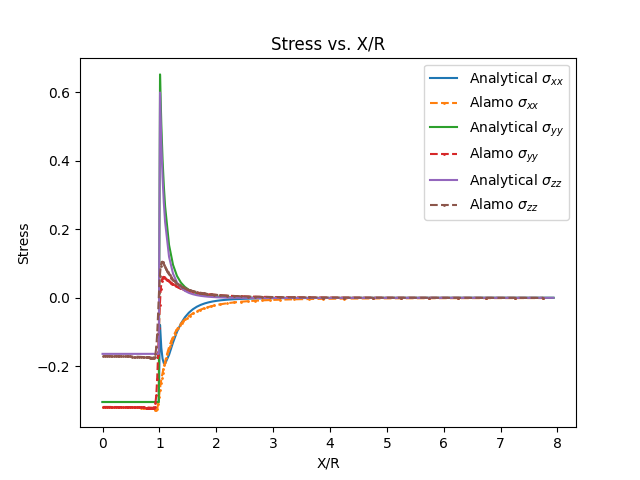
\includegraphics[width=0.45\textwidth]{images/3D_A_I_N_2_stress.png}}
  \hfill
  \subfigure[Error plot for in-homogeneous - normal strain - $E_p/E_m = 2$]{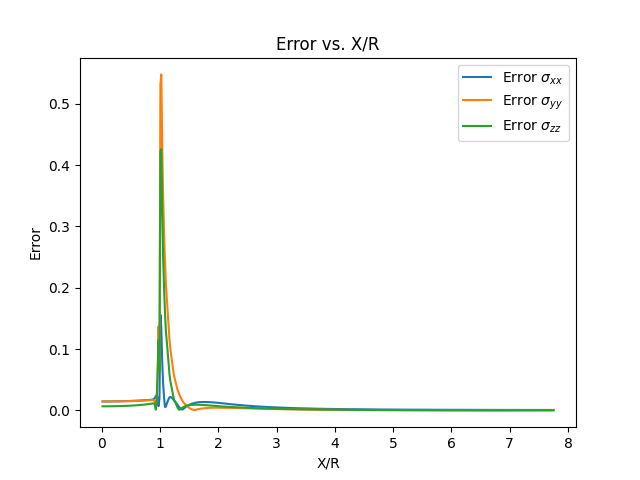
\includegraphics[width=0.45\textwidth]{images/3D_A_I_N_2_error.png}}
  \caption{Stress and error plots for Alamo - 3D - in-homogeneous - normal strain - $E_p/E_m = 2$}
\end{figure}

\begin{table}[H]
    \centering
    \begin{tabular}{|c|c|c|c|}
        \hline
        &\textbf{$\sigma_{11}$} &  \textbf{$\sigma_{22}$} & \textbf{$\sigma_{33}$}\\
        \hline
        $L_1$ & 1.502531 & 4.661978 & 3.135082 \\
        \hline
        $L_2$ & 0.259425 & 1.116279 & 0.820114 \\
        \hline 
        $L_\infty$ & 0.156018 & 0.547704 & 0.425817 \\
        \hline
    \end{tabular}
    \caption{Error in Alamo - 3D - in-homogeneous - normal strain - $E_p/E_m = 2$}
\end{table}

\paragraph{}
The input parameters, stress profile plots, error plots, and error metrics for 3D, in-homogeneous case under normal strain conditions with $E_p/E_m = 2$ for Alamo solution benchmarking are shown. Both solutions agree well in the entire range of the x-axis. There is a spike in error at the inclusion boundary.
%%%%%%%%%%%%%%%%%%%%%%%%%%%%%%%%%%%%%%%%%%%%%%%%%%%%%%%%%%%%%%%

\newpage

\subsubsection{In-Homogeneous Case - Shear Strain - $E_p/E_m = 2$}
\begin{table}[H]
    \centering
    \begin{tabular}{|c|c|c|}
        \hline
        & \textbf{Alamo} &\textbf{Analytical}\\
        \hline
        \textbf{$a_1$} & 1 & 1 \\
        \hline
        \textbf{$a_2$} & 1 & 1 \\
        \hline
        \textbf{$a_3$} & 0.5 & 0.5 \\
        \hline
        \textbf{$\nu$} & 0.3 & 0.3 \\
        \hline
        \textbf{$E_p$} & 420 & 420 \\
        \hline
        \textbf{$E_m$} & 210 & 210 \\
        \hline
        \textbf{$\epsilon_{11}$} & 0 & 0 \\
        \hline
        \textbf{$\epsilon_{22}$} & 0 & 0 \\
        \hline
        \textbf{$\epsilon_{33}$} & 0 & 0 \\
        \hline
        \textbf{$\epsilon_{12}, \epsilon_{23}, \epsilon_{31}$} & 0.001 & 0.001 \\
        \hline
        \textbf{Other} & Grid size = 32*32*32, diffuse boundary = 0.1 &  \\
        \hline
    \end{tabular}
    \caption{Input parameters for Alamo - 3D - in-homogeneous - shear strain - $E_p/E_m = 2$}
\end{table}

\begin{figure}[htbp]
  \centering
  \subfigure[Stress plot for in-homogeneous - shear strain - $E_p/E_m = 2$]{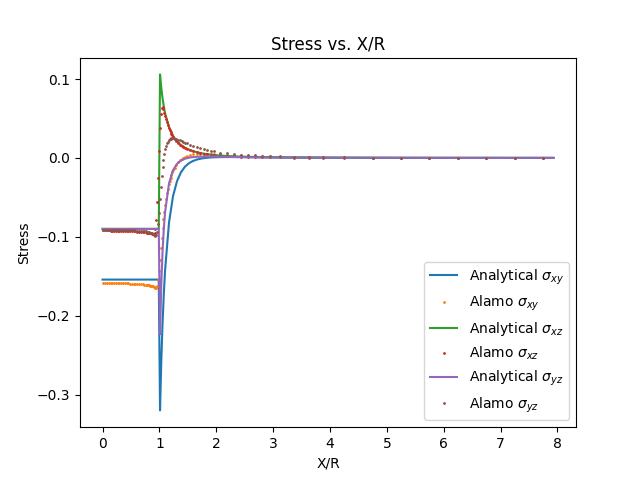
\includegraphics[width=0.45\textwidth]{images/3D_A_I_S_2_stress.png}}
  \hfill
  \subfigure[Error plot for in-homogeneous - shear strain - $E_p/E_m = 2$]{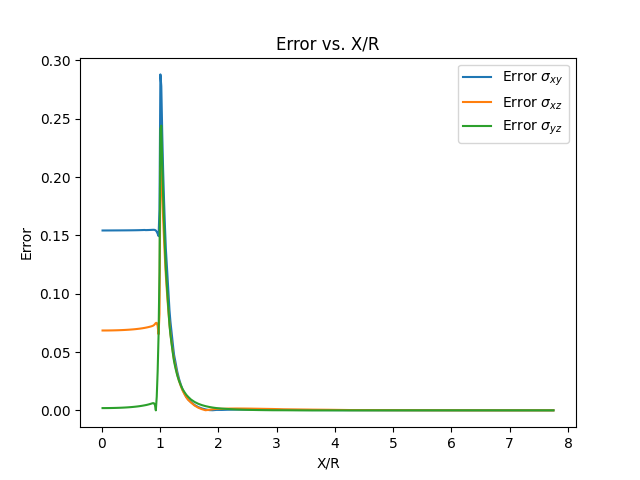
\includegraphics[width=0.45\textwidth]{images/3D_A_I_S_2_error.png}}
  \caption{Stress and error plots for Alamo - 3D - in-homogeneous - shear strain - $E_p/E_m = 2$}
\end{figure}

\begin{table}[H]
    \centering
    \begin{tabular}{|c|c|c|c|}
        \hline
        &\textbf{$\sigma_{12}$} &  \textbf{$\sigma_{23}$} & \textbf{$\sigma_{13}$}\\
        \hline
        $L_1$ & 8.609259 & 2.501291 & 4.806790 \\
        \hline
        $L_2$ & 1.167864 & 0.574369 & 0.671868 \\
        \hline 
        $L_\infty$ & 0.288054 & 0.244113 & 0.211139 \\
        \hline
    \end{tabular}
    \caption{Error in Alamo - 3D - in-homogeneous - shear strain - $E_p/E_m = 2$}
\end{table}


\paragraph{}
The input parameters, stress profile plots, error plots, and error metrics for 3D, in-homogeneous case under shear strain conditions with $E_p/E_m = 2$ for Alamo solution benchmarking are shown. Both solutions agree well outside the inclusion. There are discrete error levels inside the inclusion, which leads to an increase in error metrics. There is also a spike in error at the inclusion boundary.
%%%%%%%%%%%%%%%%%%%%%%%%%%%%%%%%%%%%%%%%%%%%%%%%%%%%%%%%%%%%%%%

\newpage

\subsubsection{In-Homogeneous Case - Normal Strain - $E_p/E_m = 0.5$}
\begin{table}[H]
    \centering
    \begin{tabular}{|c|c|c|}
        \hline
        & \textbf{Alamo} &\textbf{Analytical}\\
        \hline
        \textbf{$a_1$} & 1 & 1 \\
        \hline
        \textbf{$a_2$} & 1 & 1 \\
        \hline
        \textbf{$a_3$} & 0.5 & 0.5 \\
        \hline
        \textbf{$\nu$} & 0.3 & 0.3 \\
        \hline
        \textbf{$E_p$} & 105 & 105 \\
        \hline
        \textbf{$E_m$} & 210 & 210 \\
        \hline
        \textbf{$\epsilon_{11}$} & 0.001 & 0.001 \\
        \hline
        \textbf{$\epsilon_{22}$} & 0.001 & 0.001 \\
        \hline
        \textbf{$\epsilon_{33}$} & 0.001 & 0.001 \\
        \hline
        \textbf{$\epsilon_{12}, \epsilon_{23}, \epsilon_{31}$} & 0 & 0 \\
        \hline
        \textbf{Other} & Grid size = 32*32*32, diffuse boundary = 0.1 &  \\
        \hline
    \end{tabular}
    \caption{Input parameters for Alamo - 3D - in-homogeneous - normal strain - $E_p/E_m = 0.5$}
\end{table}

\begin{figure}[htbp]
  \centering
  \subfigure[Stress plot for in-homogeneous - normal strain - $E_p/E_m = 0.5$]{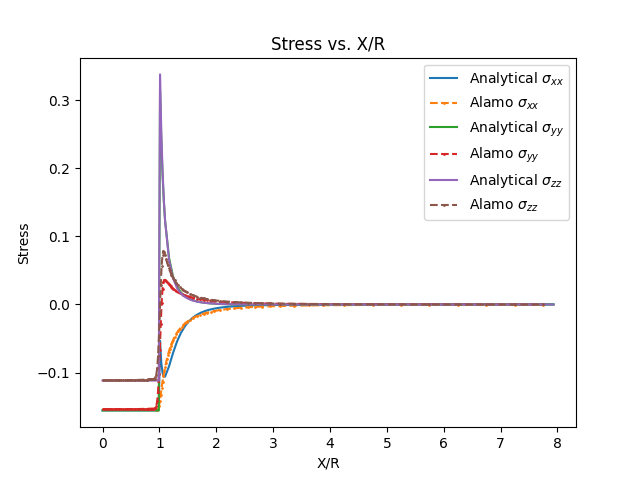
\includegraphics[width=0.45\textwidth]{images/3D_A_I_N_0.5_stress.png}}
  \hfill
  \subfigure[Error plot for in-homogeneous - normal strain - $E_p/E_m = 0.5$]{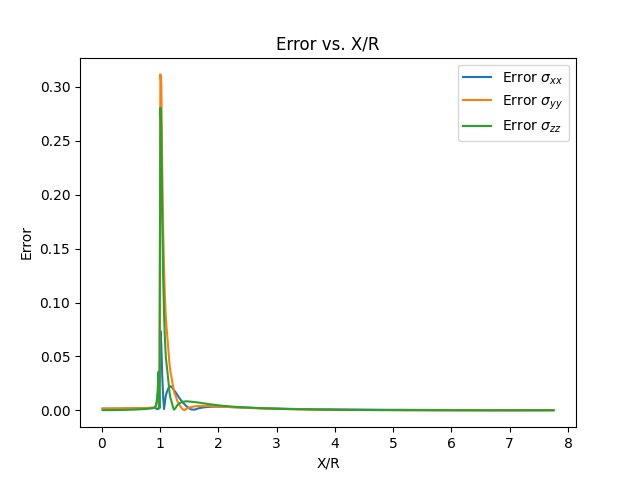
\includegraphics[width=0.45\textwidth]{images/3D_A_I_N_0.5_error.png}}
  \caption{Stress and error plots for Alamo - 3D - in-homogeneous - normal strain - $E_p/E_m = 0.5$}
\end{figure}

\begin{table}[H]
    \centering
    \begin{tabular}{|c|c|c|c|}
        \hline
        &\textbf{$\sigma_{11}$} &  \textbf{$\sigma_{22}$} & \textbf{$\sigma_{33}$}\\
        \hline
        $L_1$ & 0.591913 & 1.930380 & 1.438849 \\
        \hline
        $L_2$ & 0.124927 & 0.569664 & 0.467430 \\
        \hline 
        $L_\infty$ & 0.073675 & 0.311556 & 0.280619 \\
        \hline
    \end{tabular}
    \caption{Error in Alamo - 3D - in-homogeneous - normal strain - $E_p/E_m = 0.5$}
\end{table}

\paragraph{}
The input parameters, stress profile plots, error plots, and error metrics for 3D, in-homogeneous case under normal strain conditions with $E_p/E_m = 0.5$ for Alamo solution benchmarking are shown. Both solutions agree well in the entire range of the x-axis. There is a spike in error at the inclusion boundary.
%%%%%%%%%%%%%%%%%%%%%%%%%%%%%%%%%%%%%%%%%%%%%%%%%%%%%%%%%%%%%%%

\newpage

\subsubsection{In-Homogeneous Case - Shear Strain - $E_p/E_m = 0.5$}
\begin{table}[H]
    \centering
    \begin{tabular}{|c|c|c|}
        \hline
        & \textbf{Alamo} &\textbf{Analytical}\\
        \hline
        \textbf{$a_1$} & 1 & 1 \\
        \hline
        \textbf{$a_2$} & 1 & 1 \\
        \hline
        \textbf{$a_3$} & 0.5 & 0.5 \\
        \hline
        \textbf{$\nu$} & 0.3 & 0.3 \\
        \hline
        \textbf{$E_p$} & 105 & 105 \\
        \hline
        \textbf{$E_m$} & 210 & 210 \\
        \hline
        \textbf{$\epsilon_{11}$} & 0 & 0 \\
        \hline
        \textbf{$\epsilon_{22}$} & 0 & 0 \\
        \hline
        \textbf{$\epsilon_{33}$} & 0 & 0 \\
        \hline
        \textbf{$\epsilon_{12}, \epsilon_{23}, \epsilon_{31}$} & 0.001 & 0.001 \\
        \hline
        \textbf{Other} & Grid size = 32*32*32, diffuse boundary = 0.1 &  \\
        \hline
    \end{tabular}
    \caption{Input parameters for Alamo - 3D - in-homogeneous - shear strain - $E_p/E_m = 0.5$}
\end{table}

\begin{figure}[htbp]
  \centering
  \subfigure[Stress plot for in-homogeneous - shear strain - $E_p/E_m = 0.5$]{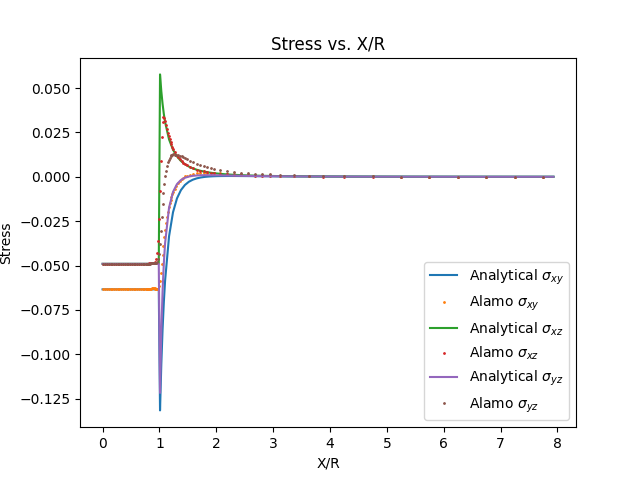
\includegraphics[width=0.45\textwidth]{images/3D_A_I_S_0.5_stress.png}}
  \hfill
  \subfigure[Error plot for in-homogeneous - shear strain - $E_p/E_m = 0.5$]{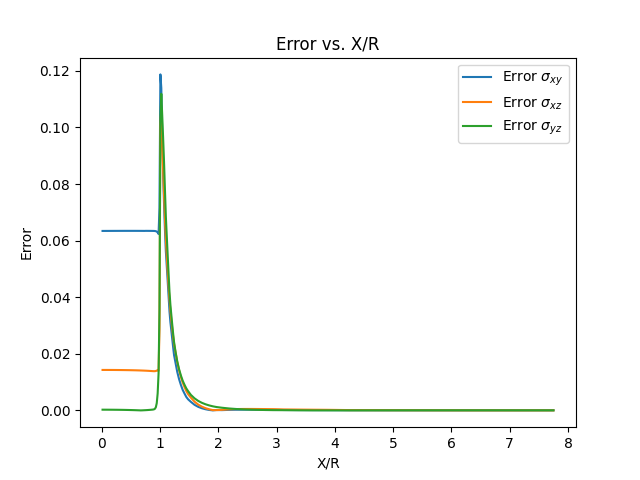
\includegraphics[width=0.45\textwidth]{images/3D_A_I_S_0.5_error.png}}
  \caption{Stress and error plots for Alamo - 3D - in-homogeneous - shear strain - $E_p/E_m = 0.5$}
\end{figure}

\begin{table}[H]
    \centering
    \begin{tabular}{|c|c|c|c|}
        \hline
        &\textbf{$\sigma_{12}$} &  \textbf{$\sigma_{23}$} & \textbf{$\sigma_{13}$}\\
        \hline
        $L_1$ & 3.531759 & 1.199266 & 1.616360 \\
        \hline
        $L_2$ & 0.479145 & 0.283594 & 0.274041 \\
        \hline 
        $L_\infty$ & 0.118736 & 0.111877 & 0.106715 \\
        \hline
    \end{tabular}
    \caption{Error in Alamo - 3D - in-homogeneous - shear strain - $E_p/E_m = 0.5$}
\end{table}

\paragraph{}
The input parameters, stress profile plots, error plots, and error metrics for 3D, in-homogeneous case under shear strain conditions with $E_p/E_m = 0.5$ for Alamo solution benchmarking are shown. Both solutions agree well outside the inclusion. There are discrete error levels inside the inclusion, which leads to an increase in error metrics. There is also a spike in error at the inclusion boundary.
%%%%%%%%%%%%%%%%%%%%%%%%%%%%%%%%%%%%%%%%%%%%%%%%%%%%%%%%%%%%%%%

\chapter{Summary and Future Work}
\paragraph{}
Analytical solutions to Eshelby's inclusion problem were derived and implemented in Python in this work. These solutions were used to benchmark those obtained from Alamo and FFT implementations. The solutions are benchmarked for both 2D and 3D cases for isotropic materials. The solutions take into consideration homogeneous as well as in-homogeneous inclusions. The solutions are also benchmarked individually for normal and shear strains. \\

The solutions benchmarked are in good agreement with error metrics, as mentioned in Chapter 3. Experiments with smaller grid sizes and larger system sizes can be tried to minimize the error metrics. This would require higher memory and computing power. \\

Since most real-life inclusions are anisotropic, analytical solutions and their implementation must be adapted to handle anisotropy. FFT solutions can handle anisotropy, but Alamo, by default, lacks an anisotropy package. Anisotropy package for Alamo using the underlying AMReX package can be developed.

\bibliography{references}

\end{document}